\documentclass[3p]{elsarticle} %review=doublespace preprint=single 5p=2 column
%%% Begin My package additions %%%%%%%%%%%%%%%%%%%

\usepackage[hyphens]{url}


\usepackage{lineno} % add
  \linenumbers % turns line numbering on

\usepackage{graphicx}
%%%%%%%%%%%%%%%% end my additions to header

\usepackage[T1]{fontenc}
\usepackage{lmodern}
\usepackage{amssymb,amsmath}
\usepackage{ifxetex,ifluatex}
\usepackage{fixltx2e} % provides \textsubscript
% use upquote if available, for straight quotes in verbatim environments
\IfFileExists{upquote.sty}{\usepackage{upquote}}{}
\ifnum 0\ifxetex 1\fi\ifluatex 1\fi=0 % if pdftex
  \usepackage[utf8]{inputenc}
\else % if luatex or xelatex
  \usepackage{fontspec}
  \ifxetex
    \usepackage{xltxtra,xunicode}
  \fi
  \defaultfontfeatures{Mapping=tex-text,Scale=MatchLowercase}
  \newcommand{\euro}{€}
\fi
% use microtype if available
\IfFileExists{microtype.sty}{\usepackage{microtype}}{}
\usepackage[]{natbib}
\bibliographystyle{plainnat}

\ifxetex
  \usepackage[setpagesize=false, % page size defined by xetex
              unicode=false, % unicode breaks when used with xetex
              xetex]{hyperref}
\else
  \usepackage[unicode=true]{hyperref}
\fi
\hypersetup{breaklinks=true,
            bookmarks=true,
            pdfauthor={},
            pdftitle={Nest shape does not affect ant colony performance against a nest invader despite altered worker movement and communication},
            colorlinks=false,
            urlcolor=blue,
            linkcolor=magenta,
            pdfborder={0 0 0}}

\setcounter{secnumdepth}{0}
% Pandoc toggle for numbering sections (defaults to be off)
\setcounter{secnumdepth}{0}


% tightlist command for lists without linebreak
\providecommand{\tightlist}{%
  \setlength{\itemsep}{0pt}\setlength{\parskip}{0pt}}




\usepackage{parskip}

\begin{document}


\begin{frontmatter}

  \title{Nest shape does not affect ant colony performance against a
nest invader despite altered worker movement and communication}
    \author[a]{Greg T. Chism}
   \ead{gchism@arizona.edu} 
    \author[b]{Alann Rathery}
  
    \author[c]{Anna Dornhaus}
  
      \affiliation[a]{Graduate Interdisciplinary Program in Entomology
and Insect Science, University of Arizona, Tucson, AZ, U.S.A.}
    \affiliation[b]{Department of Life Sciences, University of
Roehampton, London, U.K.}
    \affiliation[c]{Department of Ecology and Evolutionary Biology,
University of Arizona, Tucson, AZ, U.S.A.}
    \cortext[cor1]{Corresponding author}
  
  \begin{abstract}
  The spatial configuration or `architecture' of an animal's home can
  significantly affect the behavior of the occupant. However, the
  geometry of the occupied space may only partly be under the animals'
  control, especially if pre-existing structures are used. In social
  animals in particular, such geometry may affect not only movement of
  individuals but also facilitate (or negate) cooperative interactions.
  How then does nest architecture translate to performance and fitness?
  We address this question by manipulating internal nest shape in a
  social insect, the ant Temnothorax rugatulus. We test the defensive
  performance of ant colonies against a conspecific nest invader in two
  distinct nest shapes, where nest invasion risks brood or queen loss.
  We also compared both worker movement and interaction networks in each
  nest shape to infer the spread of information about a nest invader. We
  specifically test the following hypotheses regarding how nest shape
  may affect performance (1) by changing how well information flows
  through each nest shape; (2) by changing the physical accessibility of
  different sections of the nest, including causing `traffic jams',
  i.e., total movement blocks; or whether, alternatively, (3) nest shape
  does not impact performance against nest invaders. We found that,
  while nest shape did affect information flow and traffic jams through
  the nest, performance itself (time to remove the invader) was not
  affected by nest geometry. Our findings imply that social animals may
  be able to flexibly adapt to, and possibly compensate for, different
  spatial constraints.
  \end{abstract}
    \begin{keyword}
    Ants \sep Nest Architecture \sep Temnothorax \sep Colony
Organization \sep Nest Entrance \sep 
    Nest defense
  \end{keyword}
  
 \end{frontmatter}

\newpage

\hypertarget{introduction}{%
\section{Introduction}\label{introduction}}

Social animal architectures exist in a diversity of forms, which often
have profound effects on the social interactions of the builders and
thus their fitness (Hansell 2019). For example, kinship in social weaver
bird colonies is influenced by how clustered chambers are in collective
nests (Collias and Collias 1977; van Dijk et al., 2014), and social
organization is promoted by the physical segregation of reproductive
queens and other tasks in the architectures of naked mole rats (Tofts
and Franks 1992; Faulkes and Bennett 2001) and social insects (Anderson
1984, Wilson and Kinne 1990, Wilson 1992). In these social species,
interactions between individuals are key to essential colony functions,
such as food collection or colony defense (where recruitment plays a
critical role: Dornhaus and Powell 2009; Charbonneau et al., 2017;
Pinter-Wollman 2015; Fisher and Pinter-Wollman 2021). For example, in
ant colonies, nest chambers that are more highly connected facilitate
foraging recruitment by increasing interaction rates between returning
and potential foragers near the entrance (Pinter-Wollman 2015; Vaes et
al., 2020).

~

Social insect nests are among the most impressive examples of social
animal architecture, such as the nests of \emph{Atta} leaf-cutter ants,
which can have up to nine meters depth above or below ground and span
ten meters across (Hölldobler and Wilson 2010). So far, studies of
social insect architecture largely focus on describing their structure
and spatial configurations (Jeanne 1975; Seeley et al.,1982; Tschinkel
1987; London and Jeanne 2001; Tschinkel 2005; Tschinkel 2011). The next
interesting question, namely the fitness consequences of different types
of both built and occupied structures, has largely remained unanswered,
with the exception of thermoregulation and humidity control (Noirot and
Darlington 2000; Korb 2003; Korb 2010; Bollazi and Roces 2010; Halboth
and Roces 2017).

~

A defended, stable, nest is one of the primary characteristics of insect
sociality. Social insects generally display cooperative care of young
and reproductive division of labor, thus necessitating a nest that can
house the reproductive and the immature individuals, both of which are
often immobile - therefore colonies have been likened to a `factory
within a fortress' (Wilson 1968). These nests, with their high
concentration of individuals, are not only attractive to predators
(Nonacs 1993; Kaspari and O'Donnell 2003), but also to conspecifics:
ants are particularly fierce competitors and predators of other ants,
even their own species (Wilson 1976, Detrain, and Pasteels 1992, Foitzik
et al., 2001, Huang 2010; Bengston In Prep). Social insects are thus
under strong selective pressure to develop defensive strategies, either
through their nests or behaviors (Wilson 1976, Shorter and Rueppell
2012, Powell 2008; Powell et al., 2017). Ants exhibit many defensive
behaviors towards both preventing and removing nest invaders (Droual
1984; Detrain and Pasteels 1992; Tanner and Adler 2009; Dornhaus and
Powell 2010; Huang 2010; Tian and Zhou 2014). It is thus clear that
nests and their geometry can be a key element of social insect colony
defense. Here we are interested in how nest geometry may change the
behavior of the individuals within, and whether such changed behavior
then has consequences for colony performance, for example in the task of
defending the nest. We particularly focus on movement and interaction
networks of workers in the colony.

~

Information flow among workers in social insect is hypothesized to
influence the task performance of colonies (Ratnieks and Anderson 1999;
O'Donnell and Bulova 2007; Sendova-Franks et al., 2010; Lanan et al.,
2012; Donaldson-Matasci et al., 2013; Radeva et al., 2017). Information
flow may even be a limiting factor in effective task allocation, where
individual workers need to be informed about which tasks need doing
(Radeva et al., 2017), and information enables fast recruitment to tasks
(Donaldson-Matasci et al., 2013; Wild et al., 2021). Some tasks may
require large groups of workers to be coordinated, such as when the goal
is to overwhelm competitors at a resource (Lanan et al., 2012). Some
studies have indeed demonstrated that higher interaction rates, and thus
presumably higher information transmission, have increased task
performance (Gordon and Mehdiabadi 1999; Greene and Gordon 2007;
Pinter-Wollman et al., 2011; Pinter-Wollman 2015b; Vaes et al., 2020).
On the other hand, delays in communication may themselves be informative
and help drive adaptive organization (Ratnieks and Anderson 1999). Ant
colonies manage interaction rates for various purposes, such as reducing
disease spread through social distancing: disease spread is reduced by
clustering worker interactions and making the network diameter larger
(Stroeymeyt et al., 2018; Pusceddu et al., 2021).

~

Worker movement in the nest is also likely to be connected to colony
performance. The interaction networks of workers can be explained by
mobility in the nest (Blonder and Dornhaus 2011). Worker movement
therefore can explain task switching where workers not performing tasks
move through the nest and encounter other workers performing tasks,
where they may be recruited to a new task (Gordon and Mehdiabadi 1999,
Garrison et al., 2018). Additionally, the placement of brood affects the
spatial relationships of workers in the nest (Franks and Sendova-Franks
1992, Sempo et al., 2006; Pereira et al., 2018). For example,
\emph{Temnothorax unifasciatus} workers are hypothesized to place
different staged brood members in a ``domain of care'' directly related
to the amount of care each brood stage needs (Franks and Sendova-Franks
1992). Nest architecture additionally influences tasks related to
movement in the nest, such as in panicked evacuation: exiting at a
corner in a square nest is faster then from the middle of the wall
(Shiwakoti et al., 2011), and exiting in a circular nest is faster when
there is an occlusion at the entrance (Burd et al., 2010; Shiwakoti et
al., 2011).

~

Here we used the rock ant \emph{Temnothorax rugatulus} as a model to
answer whether nest geometry affects colony performance in two
artificial nest shapes. We examined overall performance in the
collective task of removing an experimentally introduced conspecific
nest invader, by specifically measuring latency to remove the nest
invader related to nest shape, how far the invader penetrated the nest,
and the number of defenders. We also quantified worker interaction
networks and worker movement in undisturbed (baseline) and invader
behavioral assays. We tested the hypotheses that any differences in nest
defense performance across nest shapes might be explained either by
differences in efficiency of information flow in worker interaction
networks or by differences in the dynamics of worker movement, in
particular possible worker `traffic jams'.

~

\hypertarget{methods}{%
\section{Methods}\label{methods}}

\textbf{\emph{Colony collections}}

From July to October 2017 and February to May 2018 we collected 20
colonies of \emph{Temnothorax rugatulus} on rocky, semi-steep slopes
with pine-oak-juniper forest on the Santa Catalina Mountains (GPS:
32.395, -110.688), USA, Pima County, Arizona. We found all of our
colonies in granite rock-crevices where entire colonies were collected
by aspirating after prying open the nest cavity. The colonies used here,
along with their maintenance and experimental schedule below, are the
same as in Chism et al., 2022, which shows that nest architecture
influences the spatial organization of colonies in the nest, but does
not address colony performance.

~

\textbf{\emph{Initial housing and care}}

Directly after collection, we placed colonies in generic artificial
nests resembling their natural nest sites in rock crevices. These nests
consisted of a 2-mm-thick piece of cardboard (75 mm x 50 mm x 2 mm)
between two glass panes (76.2 mm x 50.8 mm x 0.5mm), with a 2mm x 2mm
entrance at the center of one long side leading to an open nest space
(35mm x 25mm) (fig.~S1). We gave colonies food and water \emph{ad
libitum}, refreshed weekly, for the duration of their housing: water was
given through cotton ball stopped, water-filled 5 ml plastic tubes, and
food was given through both 2 ml microcentrifuge tubes of honey water
with a concentration of 1/4 teaspoon of honey per 50ml water, and
\textasciitilde1/8 (approximately 0.075g) of a fresh-frozen cockroach (
\emph{Nauphoeta cinerea} ). We further kept colonies on a 12:12 h light
cycle (8 a.m. to 8 p.m.), and constant temperature (approximately 21-24
°C). We kept all artificial nests in open-top plastic containers (11.1
cm x 11.1 cm x 3.3 cm) with walls lined with `insect-a-slip' (BioQuip
2871A, `fluon') to prevent escape.

~

\textbf{\emph{Experimental setup}}

We used a circular and a tube-shaped nest cavity (fig.~1) for the
experimental phase. We scaled the internal area of the nests to colony
size, giving colonies a consistent density and thus similar ability to
utilize their nest space. In the high-density treatment (treatment 1),
we used nest areas of 0.033 mm2 per worker. We determined this density
by examining the size of a \emph{Temnothorax rugatulus} colony that
utilized nearly all the available nest space in a pre-experimental nest
(248 workers, see fig.~S1) and doubling the area per worker to permit
flexible nest space use. We further doubled the internal nest area for
the low-density treatment (treatment 2), producing a density half as
dense as the high-density treatment (0.066 mm2 per worker). These
density treatments could result in nature from nest competition:
colonies prefer lower worker densities (Visscher 2007), so high nest
competition could result in populations occupying nests with overall
higher worker density; whereas low nest competition could allow colonies
to occupy their preferred nests. We additionally individually marked
workers with four identifying marks, one each on the head and prosoma,
and two on the gaster with multiple colors of paints (anesthetizing
workers individually with CO2 and using Testor's Pactra® paint) (see
fig.~1). We marked ants three to five days before the colony was placed
into experimental nests.

\begin{verbatim}
## here() starts at /Users/gregchism/Library/Mobile Documents/com~apple~CloudDocs/Desktop/AntColonyPerformance
\end{verbatim}

\begin{flushleft}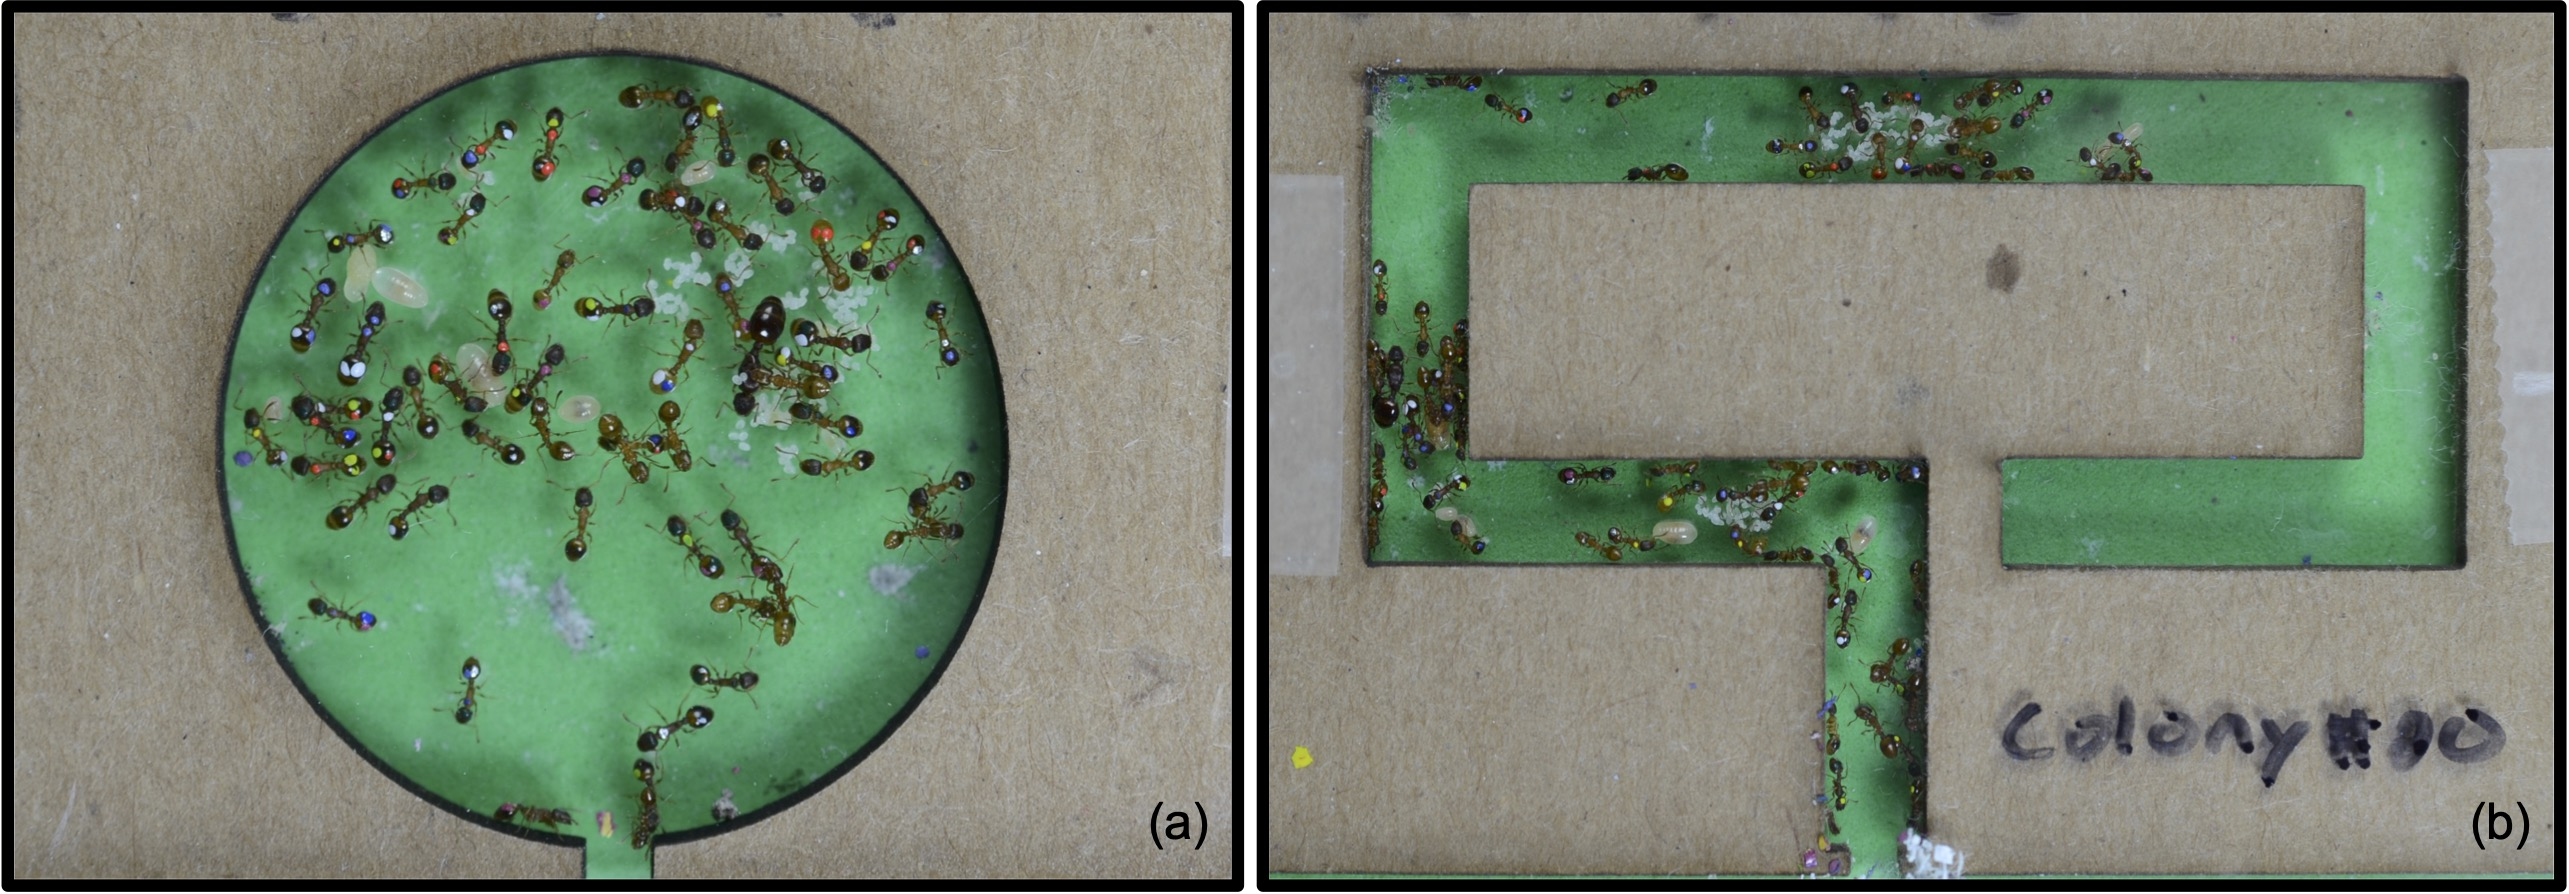
\includegraphics[width=0.75\linewidth,height=0.2\textheight]{/Users/gregchism/Library/Mobile Documents/com~apple~CloudDocs/Desktop/AntColonyPerformance/analysis/figures/Fig1} \end{flushleft}

\textbf{Figure 1}. Nest shapes used for this study, a circle (a) and
tube (b) nest.

~

\textbf{\emph{Experimental timeline}}

We had three distinct experimental phases which we employed in both
experimental density treatments. Note that half of the colonies
experienced the high worker density treatment and the other half
experienced the low worker density treatment; all colonies experienced
both nest shapes (the circular and tube-shaped nest). Food and water
were continually provided as described above.

~

\emph{Pre-experimental nest acclimation} - We gave colonies three days
to acclimate after a forced emigration (see nest defense performance,
below) into their first experimental nest. We randomly assigned nest
shapes such that ten of our colonies experienced the circle nest first
and assigned the other ten colonies the tube nest first.

~

\emph{Nest assignment I} - Following the three day acclimation period,
we photographed the nest interior of colonies in their first nest
assignment, daily at 10am for 16 days, following which we removed the
top pane of glass to expose their nest cavity, which makes emigration
into a new nest more desirable than remaining in their current exposed
nest space. We repeated the Pre-experiment acclimation procedure before
starting data collection for the second nest assignment.

~

\emph{Second pre-experimental nest acclimation} - Following the `Nest
assignment I' phase, we removed the top pane of glass to expose their
nest cavity, which makes emigration into a new nest more desirable than
remaining in their current exposed nest space. We offered a new nest of
the other type (circle or tube) and repeated the Pre-experiment
acclimation procedure.

~

\emph{Nest assignment II} - We again photographed colonies once per day
for 16 days.

~

\textbf{\emph{Video capture}}

Following the 16 day photographing period above, we recorded control
(baseline) and nest invader assay videos to capture each colony's
response to an invader and to determine how activity and communication
networks differed from the control settings. We repeated this nest
invader assay five times to assess each colony's response against an
invader (recorded at least 8 hours apart). All videos were recorded at
10am with an HD camera (Nikon D7000 with 60mm lens).

~

\emph{Nest invader assays}: We began each assay with a baseline
five-minute video to capture normal worker movements and interactions,
and then followed with a five-minute nest invader assay, where an
`invader' ( \emph{T. rugatulus} worker found foraging in the arena of
another non-experimental colony from the same population) was forcibly
inserted through the experimental nest entrance, using forceps. Note
that we used all invader assay videos where the invader was both
discernible and in the nest, for a total of N = 109 out of 180 possible
videos. Our final invader assay video sample size for each nest shape
and density combination were Circle/High = 29, Circle/Low = 28,
Tube/High = 22, Tube/Low = 30.

~

\emph{Movement tracking (ABCTracker)}: We used videos from a colony's
first invader assay in each nest for ant movement tracking. We tracked
ants in one set of five-minute baseline and invader assay videos of ten
colonies in each nest shape (five colonies from each density treatment)
for a final sample size of 20 baseline and 20 invader assay videos. We
analyzed each video using a semi-automated tracking software
(ABCTracker: abctracker.org; Rice et al., 2020), which includes an
initial marking phase to scale the distances and speeds of the ants
(producing `tracks'), followed by automated tracking and a functionality
for user corrections. We tracked the spatial positions of each worker in
each nest shape across all videos (24 fps), which the tracker outputs as
cartesian coordinates (x, y), trajectory (along a 360° axis), and
movement speed (px/s) for every frame.

\textbf{\emph{Nest sections}}

We used the image analysis software \emph{Fiji} (used for all image
analysis throughout, Schindelin et al., 2012), on screenshots from each
video to divide each nest into eight equal-area sections from the nest
entrance to the back of the nest (see fig.~S2). We chose not to use more
than eight bins because these nest section assignments were potentially
large enough to capture and segregate different worker tasks.

~

\textbf{\emph{Scaled distances in the nest}}

\emph{Distance to the nest entrance}: We calculated the shortest linear
distance within the available nest cavity from each colony member to the
nest entrance (fig.~S3). Specifically: in the circular nest, we
calculated each colony member's distance to the nest entrance (per a
reference x and y coordinate). In the tube nest, where a direct (i.e.,
straight-line) path was often not possible within the available nest
space, we found each colony member's distance to the nest section
closest to the entrance using reference coordinates for that nest
section (see Nest Sections), where we then added the shortest distance
from that nest section to the entrance through reference coordinates
(fig.~S3).

~

\emph{Distance scaling}: Actual possible distances varied across nests
since the nest dimensions were scaled to colony size to keep a
consistent worker density across colonies. To be able to compare
movement speeds of workers in relation to the nest entrance, we scaled
all calculated distances by setting the shortest distance from the back
of each nest shape to the entrance as 1, notably this scaling differs
from Chism et al., 2022 which utilized the shortest distance from the
back of the tube nest. Notably, speed was scaled only by ant-lengths
(see Traffic Jams)

~

\textbf{Nest defense performance} We assessed how long colonies took to
remove a conspecific nest invader to determine whether this was
influenced by (1) nest shape, (2) the distance the invader penetrated
the nest, or (3) worker defense recruitment.

~

\emph{Latency to remove the invader (performance)}: We quantified the
duration the invader was in the nest by subtracting the timestamps for
the insertion and removal (fully outside of the nest) of the invader.

~

\emph{Invader nest penetration}: We determined the farthest point in
which the invader penetrated the nest in each invader assay video and
then calculated the distance from the entrance by converting the
screenshot from pixels to metric using reference distances from each
image (bottom-left and top-right nest corners: top y-coordinate - bottom
y coordinate = 5cm). We then measured and scaled the invader's shortest
distance to the nest entrance using the same method as above.

~

\emph{Worker recruitment (max attacking workers)}: We used the maximum
number of workers that attacked the invader in the nest as a proxy for
worker defense recruitment. Attacking workers were identified as
individuals that were seen biting the invader for any duration.

~

\textbf{\emph{Worker social networks}}

We used the movement tracking data, five-minutes (constant over colonies
and treatments) from ABCTracker to quantify interactions between workers
in each video as unweighted adjacency matrices that were then converted
into static interaction networks. In our networks, the total number of
workers in each colony were nodes and the unweighted worker-worker
interactions were edges. We utilized unweighted networks to determine
how information might pass between workers in each of our nest shapes,
but the number of interactions (i.e.~represented by a weighted network)
were not considered because some ants were immobile and interacted the
entire video.

~

\emph{Worker interaction matrices}: We filled adjacency matrices with
either direct (workers facing one another) or indirect (any other
proximity) interactions, operationally defined as below.

~

Worker proximity: Our tracking software ABCTracker places a rectangular
box around each detected ant worker that approximates the length and
width of the worker. A worker's head was defined as the front of the
ABCTracker assigned rectangular box and the body was defined as the side
of the ABCTracker assigned rectangular box. We used this to determine
distance between and relative position of ants, in which ants could be
either direct (head-to-head) or indirect (head-to-body or body-to-body),
but note that the final networks were derived from all interactions
together. Specifically, (1) workers must be within a distance measuring
1.5 multiplied by the average box length over the entire video, or (2)
the distance from the focal worker's body to the target worker's body
must be within a distance measuring 0.5 multiplied by the average box
width of the target worker.

~

Final matrices and networks: We added all interactions and changed the
final matrix cells to a 1 for the presence of any interaction and 0 for
no interactions between worker pairs, producing unweighted adjacency
matrices for each video. We formed our networks from these final
matrices.

~

\emph{Comparative network measures}: We used several network measures to
describe the topology of our baseline and invader assay networks,
allowing us to assess whether nest shape affected the pattern of worker
interactions in baseline and invader assays.

~

Harmonic centrality (\(C\)): The distance, in terms of number of edges,
nodes are from all others in a network: equation 1 (Rochat 2009). Once
calculated, we assessed whether each worker's distance from the nest
entrance (see above) at the beginning of each video influenced these
values. Higher harmonic centrality in workers near the entrance at the
time of invasion could indicate that these workers were more central in
spreading information about the invader to all others.

\begin{enumerate}
\def\labelenumi{(\arabic{enumi})}
\tightlist
\item
  \[ C = \sum_{i \neq j}\,\frac{1}{d_{ij}}\]
\end{enumerate}

Where \emph{i} and \emph{j} represent links between node pairs, and dij
represents the shortest path between individuals \emph{i} and \emph{j}
(Dijkstra's algorithm: Dijkstra 1959). Note that disconnected nodes are
undefined and produce an infinite dij value when calculating closeness
centrality, but by taking the reciprocal of \(d_{ij}\) here these
instead are zeros.

~

Global network efficiency (\(E_{Glob}\)): We first calculated average
efficiency \(E(G)\) or the average of the inverse shortest path lengths
between \emph{i} and \emph{j} pairs in a network, which multiplies \(C\)
from equation 1 by \(\frac{1}{n(n-1)}\) because \(E(G)\) considers each
node twice as \emph{i} and \emph{j} (equation 2: Latora and Marchiori
2003; Buhl et al., 2004). For a graph \((G)\), efficiency is the ratio
between \(E(G)\) and \(E(K_n)\), where \(K_n\) is a complete graph of
order \(n\) (a graph with the same number if vertices as \(G\), but one
with \(\frac{n(n-1)}{2}\) possible edges). Global efficiency
(\(E_{Glob}\)) is therefore the average efficiency \(E(G)\) for all
paths (\(i \neq j\)) in a fully connected graph \(G\) (equation 3:
Latora and Marchiori 2003; Ek et al., 2015). Higher global efficiency
indicates that information about the conspecific nest invader could
spread faster within a network.

\begin{enumerate}
\def\labelenumi{(\arabic{enumi})}
\setcounter{enumi}{1}
\item
  \[ E(G) = \frac{1}{n(n-1)}\sum_{i \neq j}\frac{1}{d_{ij}} \]
\item
  \[ E_{Glob} = \frac{E(G)}{E(K_n)} \]
\end{enumerate}

Where \emph{n} is the total number of nodes in a network.

~

Gamma connectivity (\(\gamma\)): We calculated network connectivity as
the number of possible edges present compared to all possible in each of
our networks (the gamma index):

\begin{enumerate}
\def\labelenumi{(\arabic{enumi})}
\setcounter{enumi}{3}
\tightlist
\item
  \[\gamma = \frac{m}{3(n-2)}\]
\end{enumerate}

Where \emph{m} is the total number of edges for every network measure
and \emph{n} is the total number of nodes.

~

Reciprocity (\(r\)): We calculated the ratio of reciprocal interactions
(\(L\leftrightarrow\)) over the total interactions between workers
(\(L\)). Reciprocal interactions may be required to communicate more
complex forms of information.

\begin{enumerate}
\def\labelenumi{(\arabic{enumi})}
\setcounter{enumi}{4}
\tightlist
\item
  \[ r = \frac{L\leftrightarrow}{L} \]
\end{enumerate}

~

Transitivity (\(T_g\)): We determined the probability that the network
has interconnected adjacent nodes, represented as triplets, which
reveals the presence of tightly connected node communities. Transitivity
(also known as clustering coefficient) is the ratio between observed
triplets (\(T_0\)) over all possible triplets (\(T_1\)). We used this
measure to examine how clustered interactions in our networks are.

\begin{enumerate}
\def\labelenumi{(\arabic{enumi})}
\setcounter{enumi}{5}
\tightlist
\item
  \[ T_g = \frac{T_0}{T_1} \]
\end{enumerate}

~

\textbf{\emph{Worker activity}}

We assessed each worker's movement speed (a proxy for activity) in every
video. We standardized movement speeds as the length (pixels) of the
boxes that ABCTracker assigned to ants in each video (ant-lengths), and
then converting px/s into ant-lengths/s.

~

\emph{Movement speeds over time}: We averaged the movement speed of
every worker at two-second intervals in each video to determine how
worker movement changed in response to nest invasion. Temnothorax
rugatulus are slow moving ants (many workers are always inactive:
Charbonneau et al., Dornhaus 2017) so we averaged movement in a
two-second window to reduce redundancy and noise in the data.

~

\emph{Movement speeds over distance from the nest entrance}: We averaged
all worker movement speeds within 0.05 scaled distance from the entrance
bins (from 0-1, see Invader nest penetration above) to determine how
worker movement speed relates to distance from the nest entrance - see
above for distance calculations.

~

\textbf{\emph{Traffic jams}}

We estimated the likelihood of traffic jams in the nest by examining the
variation in worker movement speeds over both assay time and nest space.
Variation in speed across time could represent time periods of slow and
fast movement, and variation in speed across space could represent parts
of the nest that movement bottlenecked in, either indicating that
traffic jams occurred.

\emph{Traffic jams across space}: We calculated and averaged
interquartile ranges (3rd quartile - 1st quartile) for all baseline and
invader assay video two-second intervals from above to examine movement
speed variability over time. Our final data sets were one average
two-second interval interquartile range value for each video (N = 40
videos). Higher variation in movement across present at specific areas
of the nest could indicate that slow moving workers are restricting
traffic flow, whereas low variation could indicate that traffic flows
freely throughout the nest.

~

\emph{Traffic jams over time}: We calculated and averaged the
interquartile ranges from each 0.05 scaled distance bin from above to
examine the variability in movement speeds across nest space in each
video. Our final data sets were one average 0.05 scaled distance bin
interquartile range value for each video (N = 40 videos). Higher
movement speed variation (larger average interquartile ranges) would
indicate, for example, that some workers moved very slowly (or not at
all) and others more quickly throughout the assay. This high variation
in worker movement speeds could indicate that traffic jams are
occurring, whereas less variation (or more similar) movement speeds
could indicate that traffic flows freely.

~

Worker density in nest sections and traffic: We determined how worker
density (number of workers in nest sections) related to worker movement
speeds as another indicator for traffic jams, such that higher worker
densities could restrict worker movement in individual nest sections.

~

\textbf{\emph{Data processing}}

We conducted all data processing using the statistical software R
(v4.1.1; R Core Team 2017) and RStudio (v1.2.5042; Allaire 2012),
specifically the tidyverse language (`tidyverse' v1.3.1: Wickham et al.,
2019). All original data and analysis scripts are publicly available on
github at https://github.com/Gchism94/AntColonyPerformance

~

\emph{Network generation}: We both produced and analyzed our networks
using the R package `igraph' (v1.2.6; Csardi and Nepusz 2006), except
harmonic centrality, which was calculated using the R package `CINNA'
(v1.1.53; Ashtiani et al., 2019).

~

Factors influencing colony performance: We used linear mixed effects
(henceforth LME) models to test whether nest shape, invader nest
penetration (max scaled distance from the nest entrance), and defense
recruitment (max attacking workers) affected colony performance in
removing a conspecific nest invader. We conducted these models with the
R package `lme4' (v1.1-27.1; Bates et al., 2014), where p values were
calculated through the R package `lmerTest' (v3.1-3; Kuznetsova et al.,
2017). Our LMEs here and below had colony identification (henceforth
colony ID) as a random effect, and by comparing the variation explained
by the fixed effects alone (marginal R\textsuperscript{2+}) and with the
random effect included (conditional R\textsuperscript{2+}), we
determined the amount of variation that colony ID explained (marginal
and conditional R\textsuperscript{2+} values calculated through the R
package `MuMIn' (v1.43.17; Bartoń 2020).

~

\emph{Comparative network measures} Harmonic centrality and distance to
the entrance: We used a linear regression to test whether worker scaled
distance to the nest entrance at the beginning of the invader assay
affected the number of interactions workers had in networks (harmonic
centrality) in every video. We specifically examined the individual
terms and two-way interaction combinations between worker scaled
distance to the nest entrance, nest shape, and experimental trial, and
the three-way interaction between these terms.

~

Network efficiency: We used a linear regression to test the global
efficiency of worker interaction networks in each nest shape,
experimental trial, and the interaction between the two terms. We log
transformed network efficiency to account for all values being extremely
small, producing a strongly right-tailed data distribution.

~

We used linear regressions to determine how our comparative network
measures gamma connectivity, reciprocity, and transitivity (clustering)
differed across nest shape, experimental trial, and the interaction
between the two terms.

~

\emph{Worker activity}: We used LME models to examine both average
worker speed (two-second intervals) across our nest shapes and
experimental trials.

~

\emph{Worker traffic jams over time and nest space}: We used LME models
to examine both the variation (average interquartile ranges) in worker
movement speed through time (two-second intervals) and in average worker
speed (two-second intervals) in relation to worker scaled distance from
the nest entrance (0.05 scaled distance from the entrance intervals) in
our nest shapes and experimental trials.

~

\emph{Worker density in nest sections and traffic}: We used a LME model
to examine worker density (proportions in each nest section) in the nest
affects worker movement speeds. We considered the relationships between
average worker movement speeds against worker density, and the
interactions between worker density and nest shape, worker density and
experiment trial, and the three-way interaction between worker density,
nest shape, and experimental trial.

~

\hypertarget{results}{%
\section{Results}\label{results}}

\textbf{\emph{Colony performance against a nest invader}}

Invader removal was influenced by invader penetration and colony defense
recruitment We found that nest shape does not affect invader removal
time (seconds) (\(p = 0.746\), fig.~2a, table S1), but invaders were
removed slower in relation to both farther invader nest penetration
(\(p < 0.001\); fig.~2b, table S2) and higher worker recruitment
(\(p < 0.001\); fig.~2c, table S3). Therefore, invader removal time was
slower both when the invader penetrated farther into the nest and more
workers were recruited to remove the invader. The mean \(\pm\) standard
deviation for invader removal time was \(199\pm314\) seconds in the
circular nest and \(181\pm274\) seconds in the tube nest.

\begin{flushleft}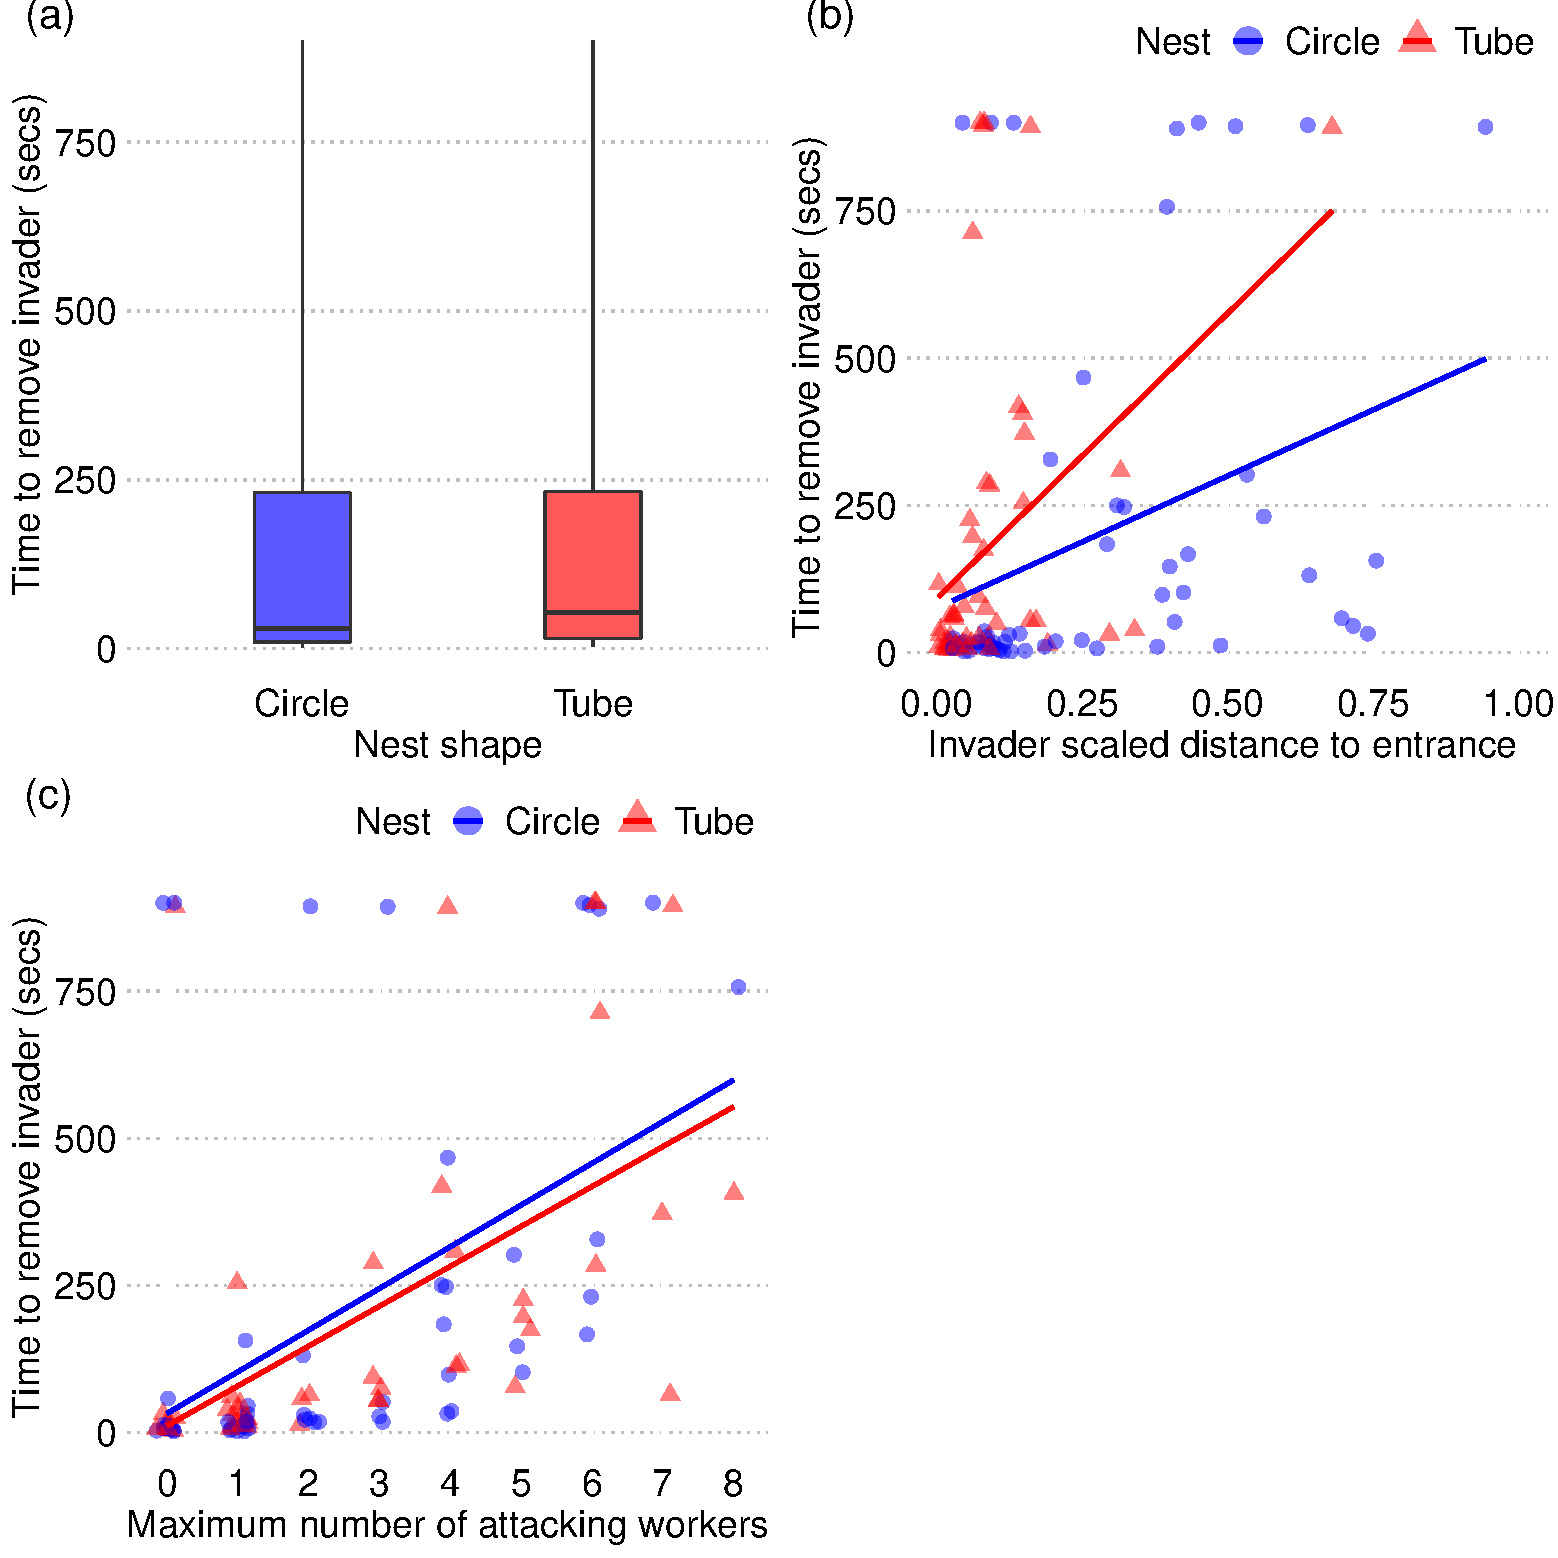
\includegraphics[width=0.95\linewidth,height=0.75\textheight]{/Users/gregchism/Library/Mobile Documents/com~apple~CloudDocs/Desktop/AntColonyPerformance/analysis/figures/Fig2} \end{flushleft}

\textbf{Figure 2}. Effect of nest shape (a), worker nest penetration
(b), defense recruitment (c) on invader removal time. The data is from
all replications of the invader assay for each colony, in each nest
shape where the invader was discernible (up to five replicates). In all
plots, data points represent one video and are jittered.

~

Colony identification explained substantial invader removal performance
model variation We found that colony ID explained 3.2\% (virtually all)
of model variation predicting the effect of nest shape on invader
removal (Marginal R\textsuperscript{2+} = 0.001, Conditional
R\textsuperscript{2+} = 0.033, table S1). We also found that colony ID
explained 6.6\% of model variation predicting the effect of nest shape
and worker nest penetration on invader removal time (Marginal
R\textsuperscript{2+} = 0.109, Conditional R\textsuperscript{2+} =
0.175, table S2), and 2.4\% of model variation towards the effect of
worker recruitment and nest shape on invader removal time (Marginal
R\textsuperscript{2+} = 0.292, Conditional R\textsuperscript{2+} =
0.316, table S3).

~

\textbf{\emph{Worker interaction networks}}

\emph{Workers near the entrance when the invader was introduced were
more central in networks}

We found that workers had higher harmonic centrality values (interacted
with more individuals) when they were closer to the nest entrance at the
time the invader was introduced (\(p < 0.001\); fig.~3a-d, table S4). We
also found that workers had higher harmonic centrality in both the
circular nest (\(p < 0.001\); fig.~3, table S4), and baseline assay
(\(p < 0.001\); fig.~3, table S4). We however found that the negative
relationship between worker distance to the nest entrance and harmonic
centrality was stronger in the invader assay (\(p = 0.011\); fig.~3,
table S4). Therefore, workers near the entrance interacted with more
workers particularly during nest invasion.

\begin{flushleft}\includegraphics[width=0.8\linewidth,height=0.6\textheight]{/Users/gregchism/Library/Mobile Documents/com~apple~CloudDocs/Desktop/AntColonyPerformance/analysis/figures/Fig3a_d} \end{flushleft}

\begin{flushleft}\includegraphics[width=0.8\linewidth,height=0.6\textheight]{/Users/gregchism/Library/Mobile Documents/com~apple~CloudDocs/Desktop/AntColonyPerformance/analysis/figures/Fig3e_f} \end{flushleft}

\begin{flushleft}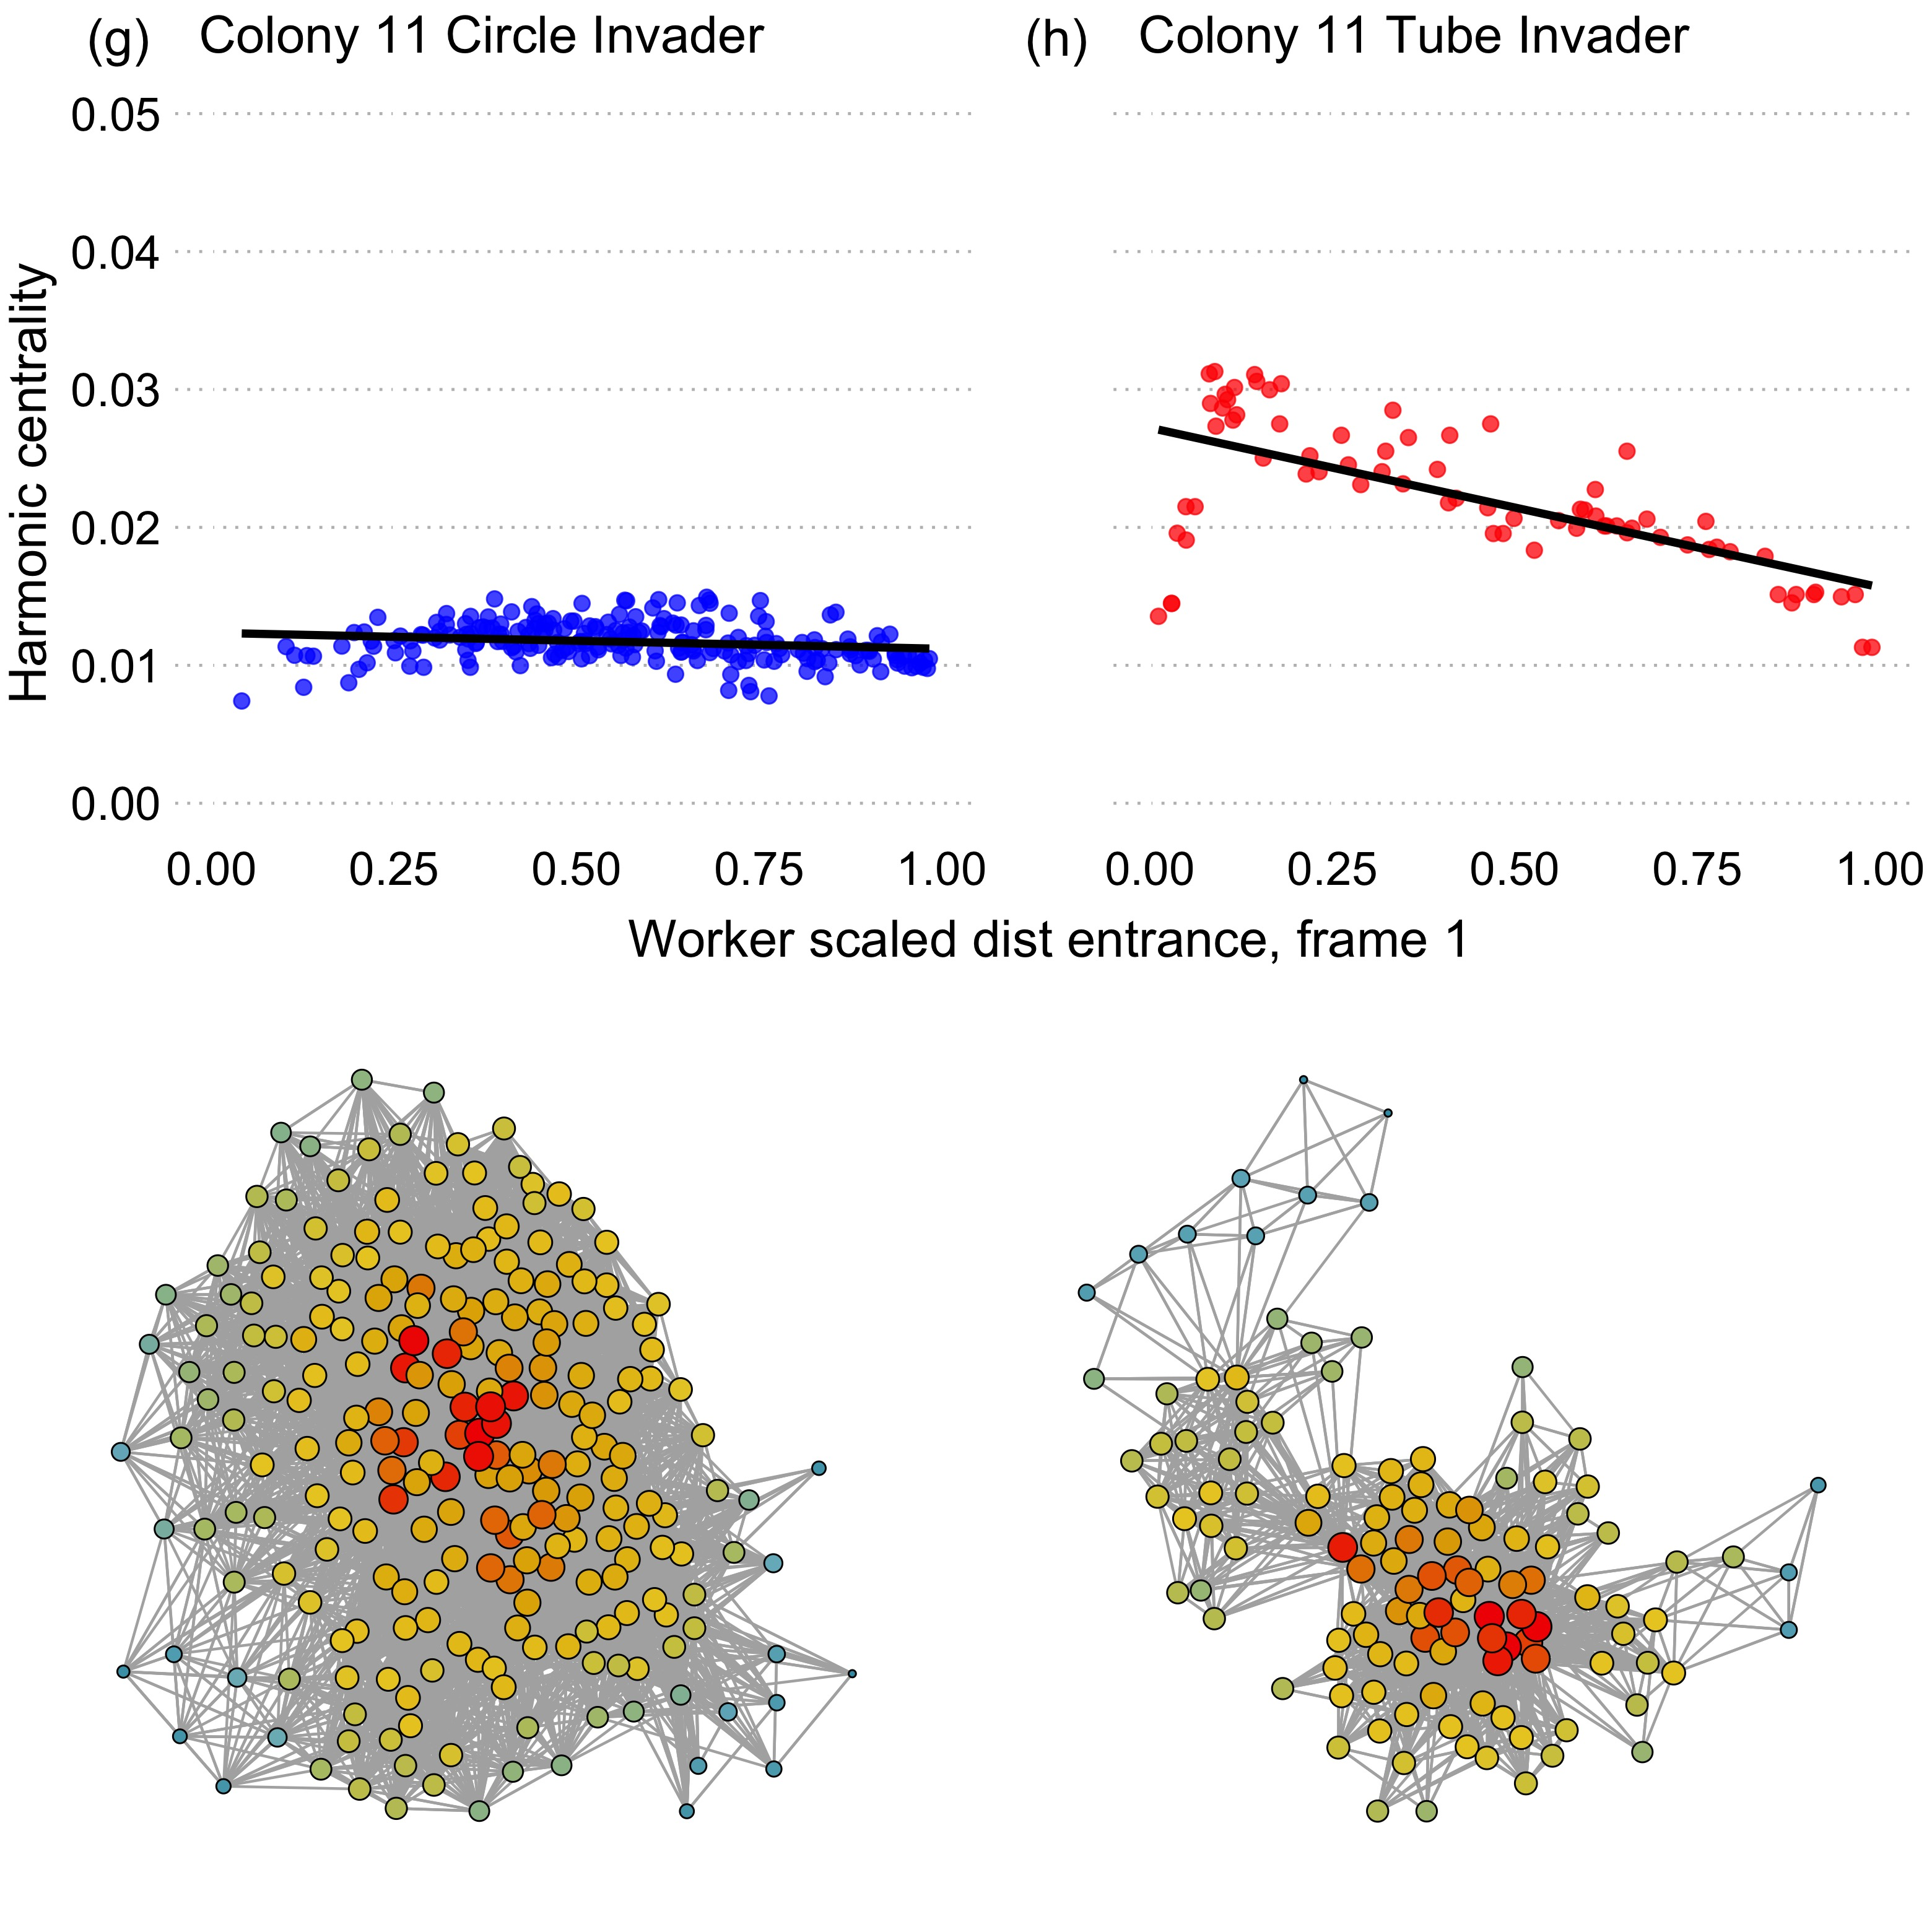
\includegraphics[width=0.8\linewidth,height=0.6\textheight]{/Users/gregchism/Library/Mobile Documents/com~apple~CloudDocs/Desktop/AntColonyPerformance/analysis/figures/Fig3g_h} \end{flushleft}

\textbf{Figure 3}. Relationship between worker distance to the entrance,
considered at frame 1 when the nest invader was introduced (x-axis) and
worker network centrality (harmonic centrality, y-axis) for all colonies
(a-d) and colony no. 11 (e-h). Worker interaction networks for colony
no. 11 (e-h) shows workers as nodes (cooler smaller nodes representing
smaller values of harmonic centrality and warmer larger nodes represent
larger values) and interactions between worker pairs as edges (gray
lines).

~

\emph{Nest shape affected how efficient information spread through
worker interaction networks}

We found that worker interaction networks were more efficient at
spreading information in the tube nest (\(p = 0.021\); fig.~4, table
S5). However, network efficiency did not differ across experimental
trials (\(p = 0.138\); fig.~4, table S5). Therefore, information
possibly spreads faster in the tube nest, but nest invasion did not
change this relationship.

\begin{flushleft}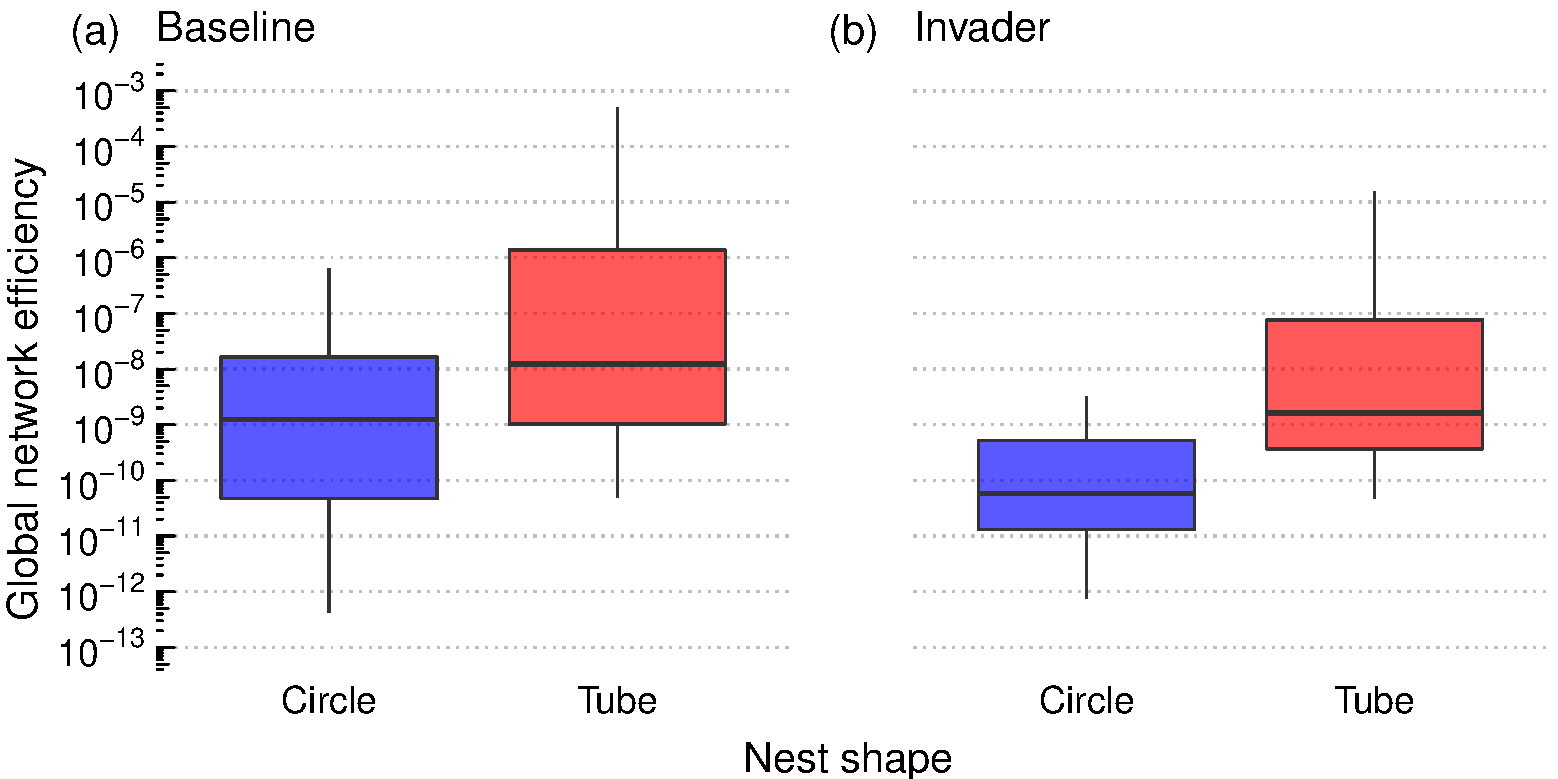
\includegraphics[width=0.9\linewidth,height=0.35\textheight]{/Users/gregchism/Library/Mobile Documents/com~apple~CloudDocs/Desktop/AntColonyPerformance/analysis/figures/Fig4} \end{flushleft}

\textbf{Figure 4}. Network efficiency and nest shape in the baseline (a)
and invader (b) assays. Global efficiency determines how effectively
information would flow through the network - log scaled, as the values
are very small, and the data are severely right-tailed.

~

\emph{All worker interaction networks were similarly connected}

We found that gamma connectivity did not differ with nest shape
(\(p = 0.060\); fig.~S4, table S6), or experimental trial
(\(p = 0.275\); fig.~S4, table S6).

~

\emph{Worker interactions were more reciprocal in the invader assay}

We found that network reciprocity did not differ with nest shape
(\(p = 0.821\); fig.~S5, table S7), but was overall higher in the
invader assay (\(p = 0.002\); fig.~S5, table S7).

~

\emph{All worker interaction networks were similarly clustered}

We found that network transitivity did not differ across nest shapes
(\(p = 0.344\); fig.~S6, table S8), or experimental trials
(\(p = 0.946\); fig.~S6, table S8).

\textbf{\emph{Worker activity}}

\emph{Worker movement speeds were different across both nest shape and
experimental trial}

We found that average worker movement speeds over our five-minute videos
were higher in the tube nest shape (\(p < 0.001\); fig.~5, table S9) and
invader assay (\(p < 0.001\); fig.~5, table S9). Further, average worker
speeds were higher in the beginning of invader assay videos in the
circular nest compared to the tube nest (\(p < 0.001\); fig.~5, table
S9). Therefore, workers moved overall faster in the tube nest and
invader assay. The mean \(\pm\) standard deviation for the observations
of two-second average worker speeds in our videos was \(31567\pm6525\)
for the baseline assay and \(29935\pm5780\) for the invader assay.

\begin{flushleft}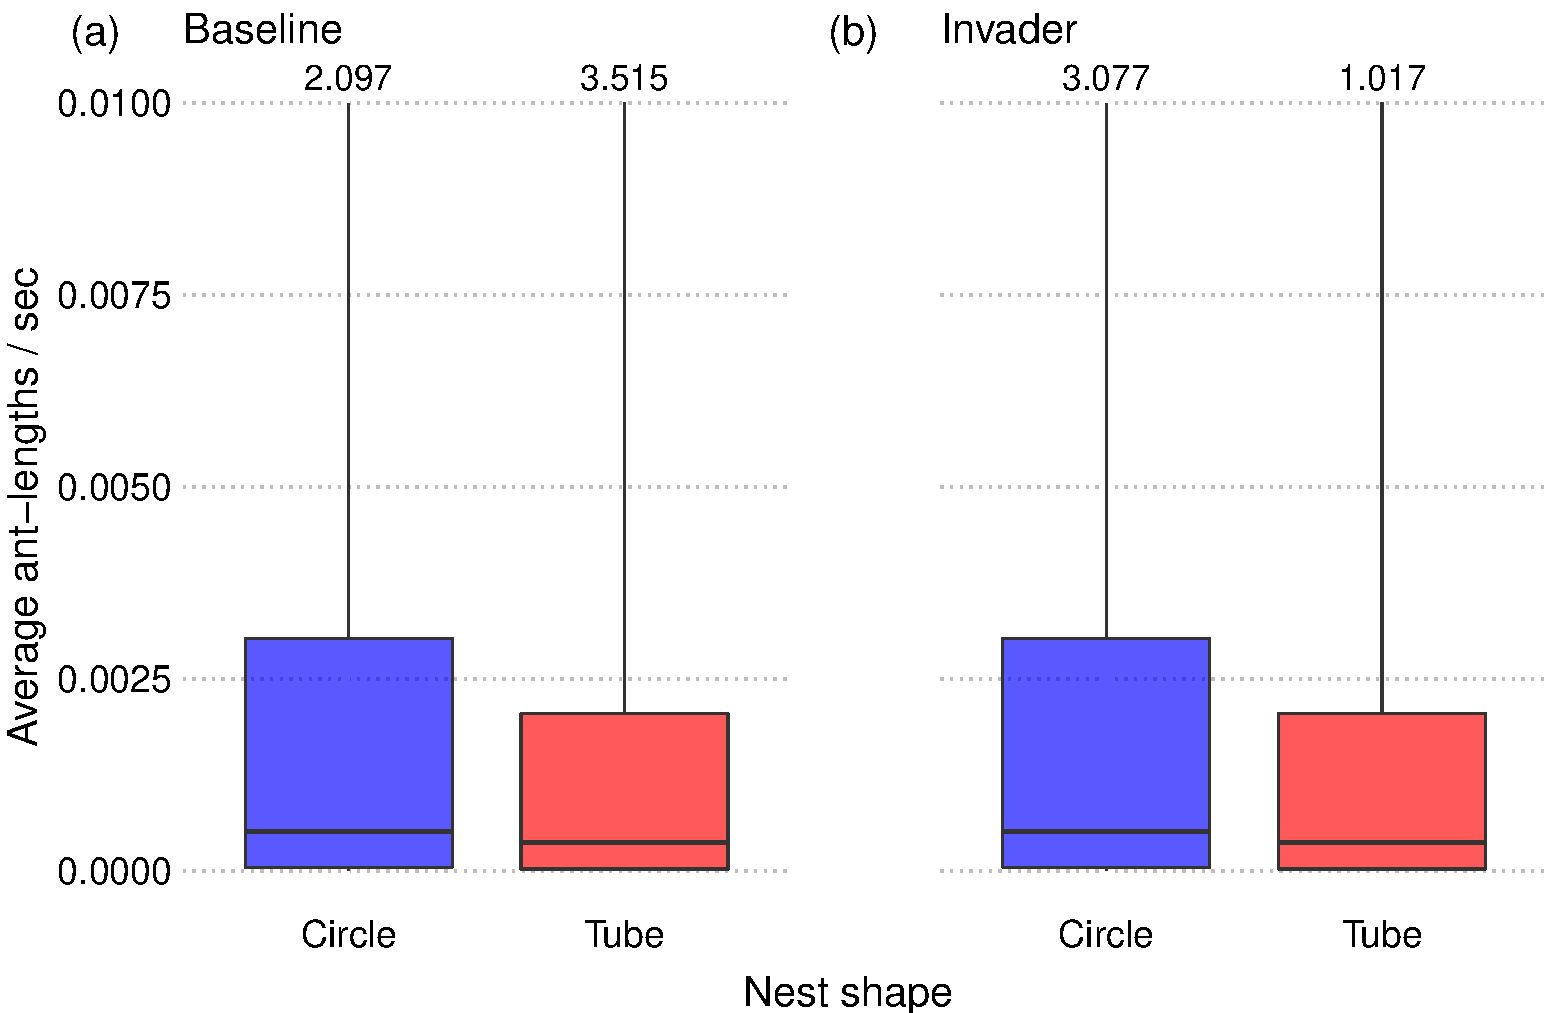
\includegraphics[width=0.9\linewidth,height=0.45\textheight]{/Users/gregchism/Library/Mobile Documents/com~apple~CloudDocs/Desktop/AntColonyPerformance/analysis/figures/Fig5} \end{flushleft}

\textbf{Figure 5}. Average worker movement speeds (ant-lengths/second)
across both nest shape and experimental trial. Each data point is the
average speed of each worker over two-seconds. Here and in all following
box plots, boxes represent first and third quartiles, bars represent the
median, whiskers are the data range, and numbers represent the max value
for that box plot. Note that the y-axis is limited at 0.01 average
ant-lengths/second.

~

\emph{Traffic jams through nest space were more likely in the invader
assay}

We found that the variation (average two-second IQR) in worker movement
speed across our five-minute videos was much higher in the invader assay
(\(p < 0.001\); fig.~6, table S10). We also found that the tube nest had
higher movement speed variation in the baseline assay, but variation in
invader assays was higher in the circular nest (\(p < 0.001\); fig.~6,
table S10). Therefore, traffic jams through nest space likely occurred
more during nest invasion, but especially so in the circular nest.

\begin{flushleft}\includegraphics[width=0.9\linewidth,height=0.45\textheight]{/Users/gregchism/Library/Mobile Documents/com~apple~CloudDocs/Desktop/AntColonyPerformance/analysis/figures/Fig6} \end{flushleft}

\textbf{Figure 6.} Traffic jams: variation in ant speed through nest
space. The average interquartile range of average movement speeds within
two-second bins for all colonies across nest shape and experimental
trial. Higher movement speed variation at specific time points could
indicate that very slow moving (or stationary) workers cause traffic
jams throughout the nest periodically. There is one point per colony,
and overarching boxplot shows variation among colonies.

~

\emph{Colony identification explained half of the variation in raw
worker movement speed}

We found that colony ID explained 6.7\% of the average worker speed over
time model variation (Marginal R\textsuperscript{2+} = 0.052,
Conditional R\textsuperscript{2+} = 0.119, table S9), and 0\% of the
average interquartile ranges of worker speeds over time model variation
(table S10).

~

Traffic jams through time were more likely in the invader assay We found
that the variation (average 0.05 scaled distance from the entrance
interval IQR) was higher in the circular nest shape (\(p = 0.036\);
fig.~7, table S11), and was significantly higher in the invader assay
(\(p < 0.001\); fig.~7, table S11). We also found that the relationship
between nest shape and worker movement speeds throughout the nest was
not different in each experimental trial (\(p = 0.107\); fig.~7, table
S11). Therefore, there were more traffic jams in the circular nest over
time, but especially so in the invader assay. The mean \(\pm\) standard
deviation for the number of workers in each 0.05 scaled distance from
the nest entrance interval was \(299\pm119\) for the baseline assay and
\(138\pm64.4\) for the invader assay.

\begin{flushleft}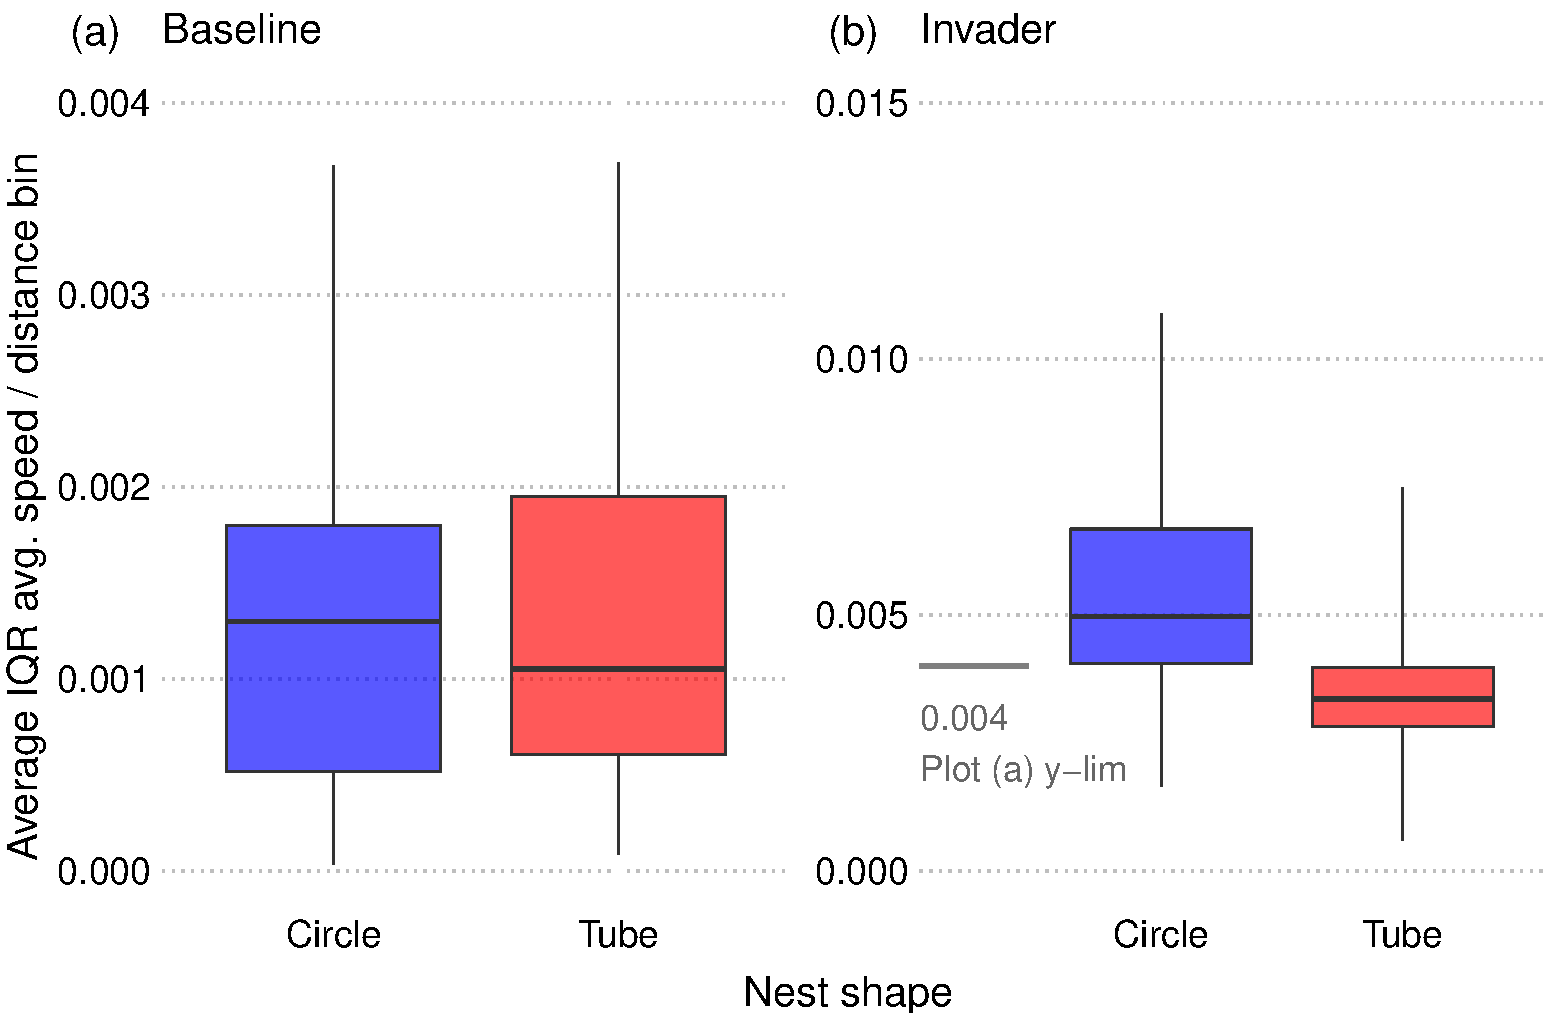
\includegraphics[width=0.9\linewidth,height=0.45\textheight]{/Users/gregchism/Library/Mobile Documents/com~apple~CloudDocs/Desktop/AntColonyPerformance/analysis/figures/Fig7} \end{flushleft}

\textbf{Figure 7.} Traffic jams: variation in speed across ants through
time. The average interquartile range of average movement speeds in each
0.05 distance bin (see fig.~S8), ranging from 0 (the entrance) to 1 (the
back of the nest), for all colonies across nest shape and experimental
trial. Higher movement variation in specific areas of the nest could
indicate where slow moving workers are restricting traffic flow over
time. Note that the y-axis limit for the baseline assay (a) is
represented in the invader assay panel (b) as a gray horizontal line.

~

\emph{Worker density promotes slower worker movement (traffic jams) in
nest sections}

We found that average worker movement speed (two-second intervals) was
lower in nest sections with higher proportions of workers
(\(p < 0.001\); fig.~8, table S12). We further found that this negative
relationship was stronger in the tube nests (\(p < 0.001\); fig.~8 table
S12), and in the invader assay (\(p < 0.001\); fig.~8, table S12).
Therefore, traffic jams occurred more over time in nest sections with
higher worker density. The mean \(\pm\) standard deviation of the
proportion of workers in nest sections was \(0.231\pm0.248\) for the
baseline assay and \(0.238\pm0.252\) in the invader assay.

\begin{flushleft}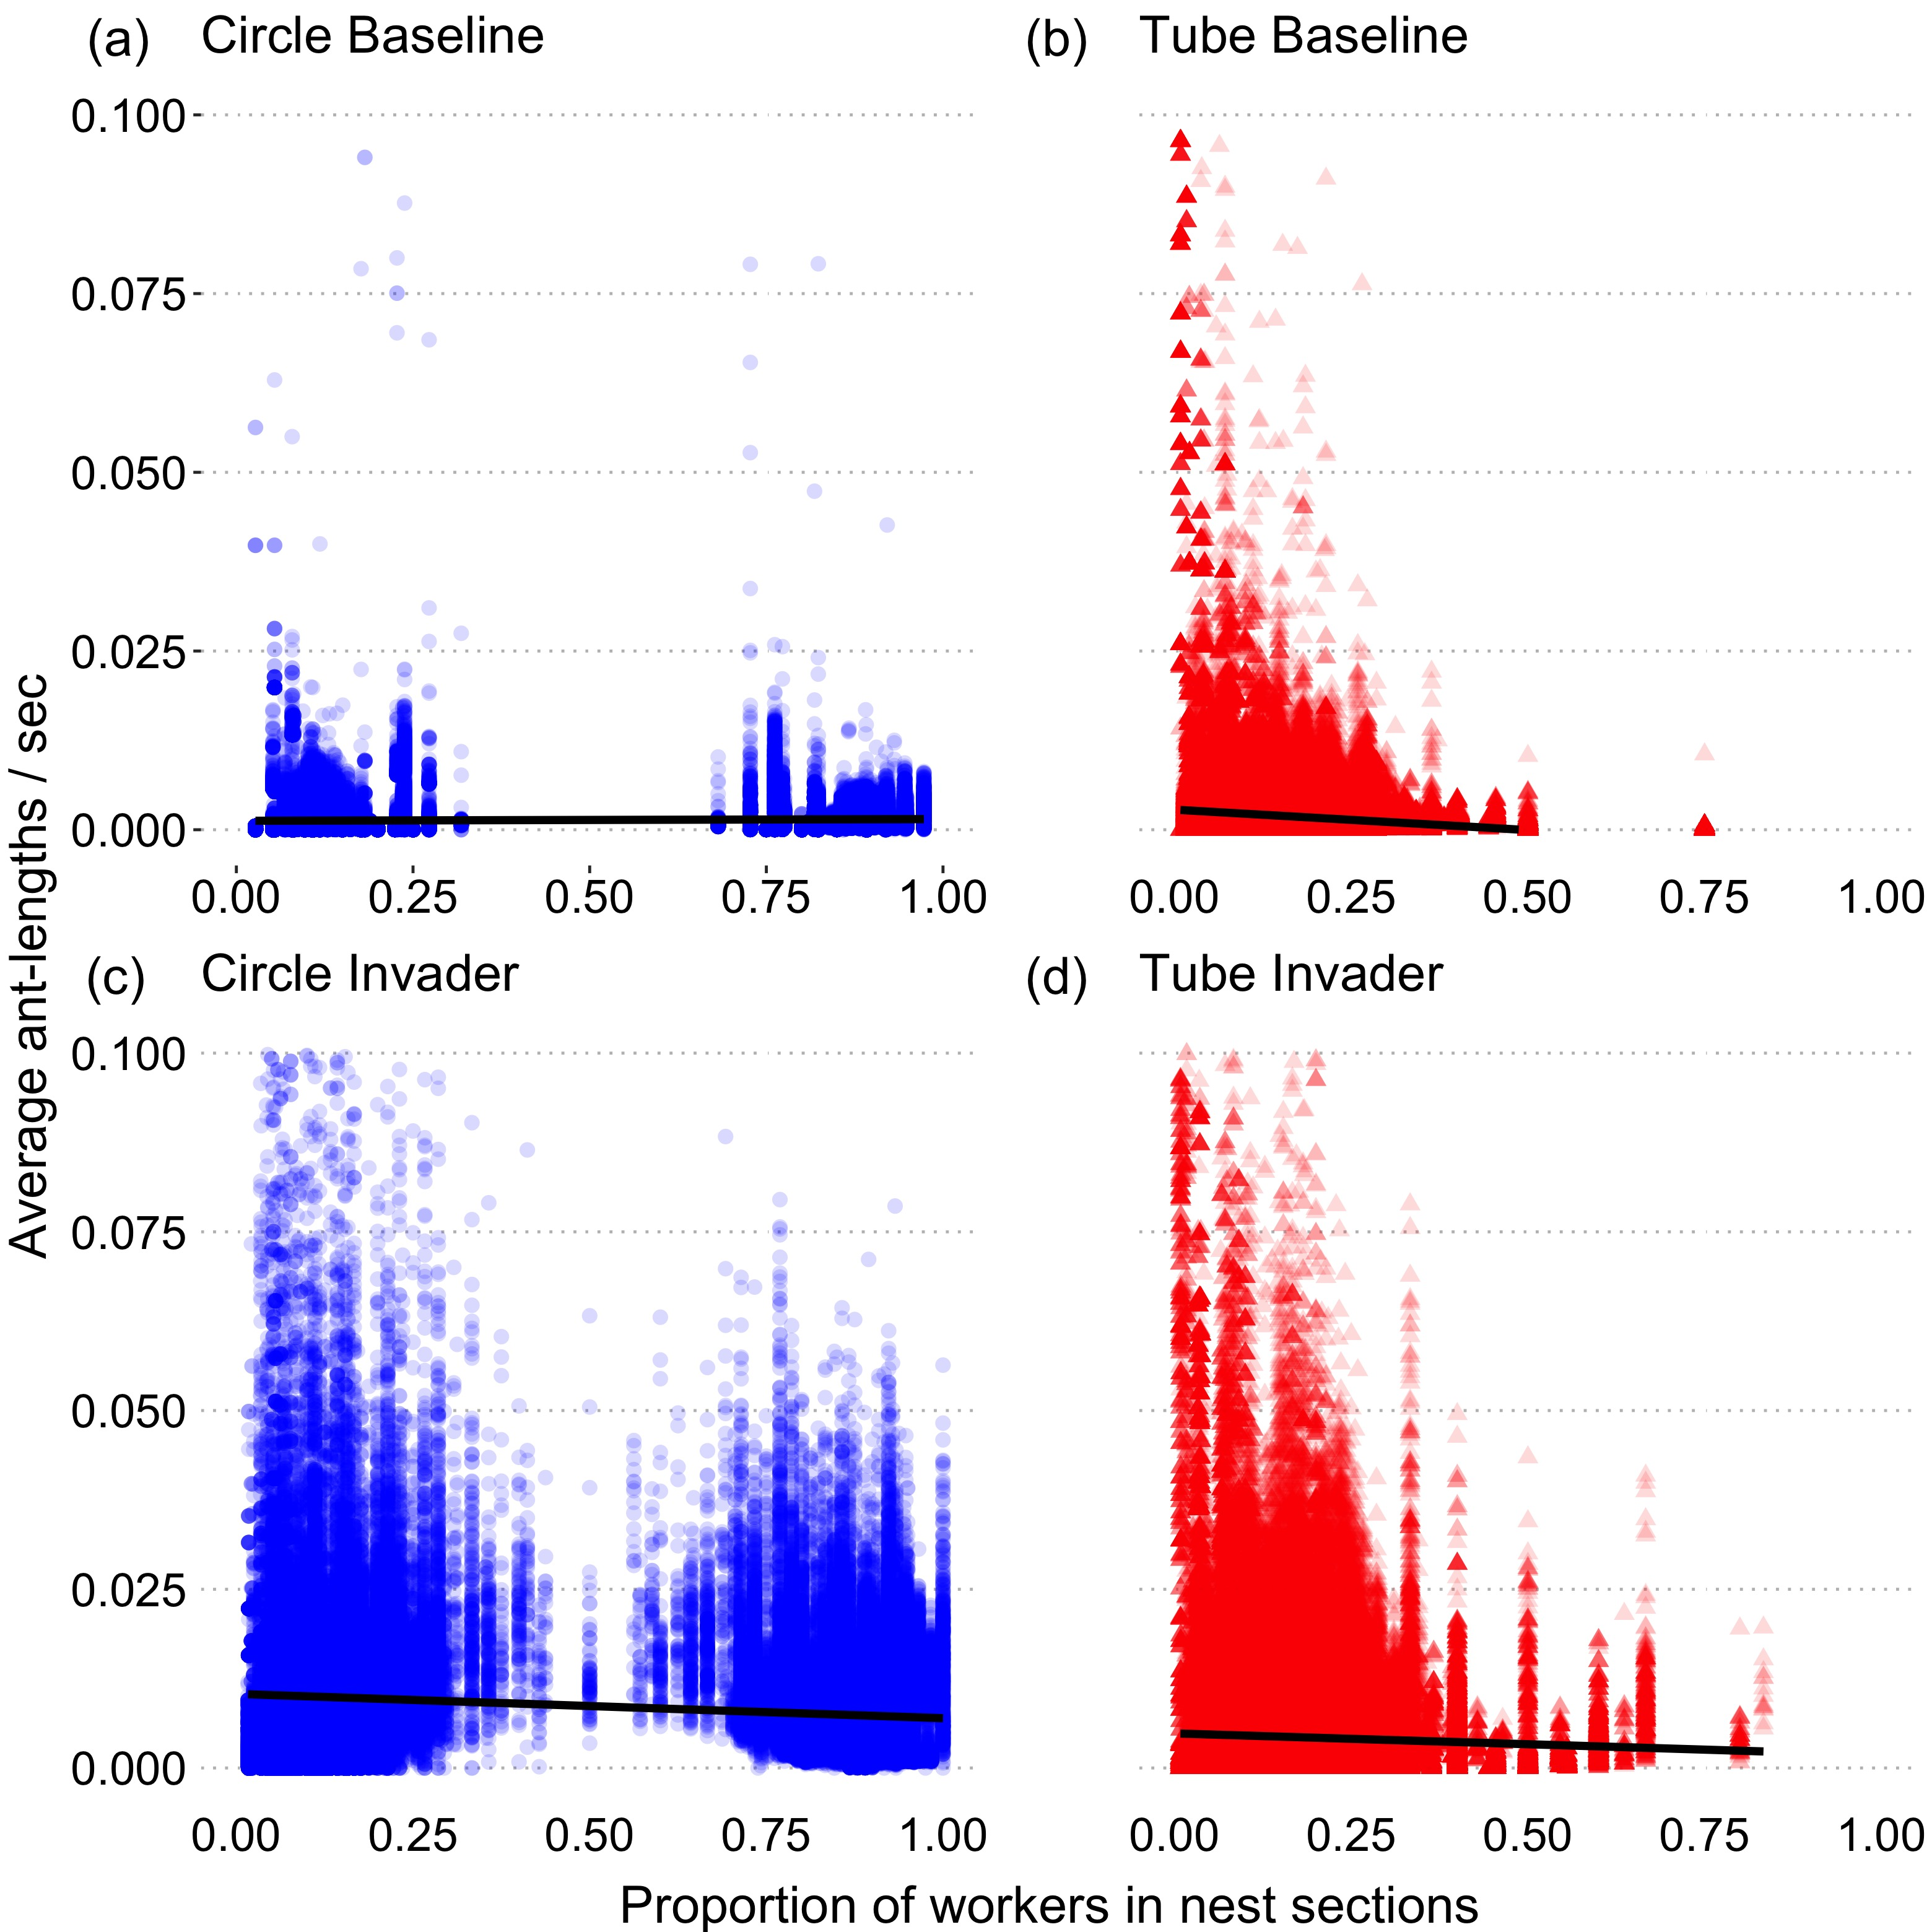
\includegraphics[width=0.8\linewidth,height=0.6\textheight]{/Users/gregchism/Library/Mobile Documents/com~apple~CloudDocs/Desktop/AntColonyPerformance/analysis/figures/Fig8} \end{flushleft}

\textbf{Figure 8.} The relationship between worker density in nest
sections and worker movement speed in each nest shape and experimental
trial. Each nest is binned into eight even area sections where the
proportion of workers in each nest section is determined to approximate
density throughout the nest. Each data point is movement speed
determined at every time step, black lines represent linear fits.

~

\emph{Colony identification slightly influenced models predicting
traffic jams over time}

We found that colony ID explained 5.9\% of the model variation for
average interquartile ranges of average worker speeds in 0.05 scaled
distance to the entrance bins (Marginal R\textsuperscript{2+} = 0.464,
Conditional R\textsuperscript{2+} = 0.523, table S11). We further found
that colony ID explained 3.8\% of the model variation examining for
worker density in the nest and average worker movement speeds (Marginal
R\textsuperscript{2+} = 0.143, Conditional R\textsuperscript{2+} =
0.182, table S12).

~

\hypertarget{discussion}{%
\section{Discussion}\label{discussion}}

Nest architecture does not influence \emph{Temnothorax rugatulus} ant
colony performance against a conspecific nest invader: we found that the
removal of nest invaders was slower when invaders penetrated the nest
farther (fig.~2b) and when more defending workers were recruited
(fig.~2c), but invader removal was not influenced by nest shape
(fig.~2a). We contrastingly found significant nest shape related
differences in how well assumed information about the nest invader may
spread throughout worker interaction networks (figs. 3,4). We also show
that traffic jams may occur during nest invasion, represented by higher
worker movement variation both through nest space (fig.~6) and worker
density in nest sections (fig.~8) that may bottleneck worker movement
over time. Therefore, nest shape influences the movement and
communication of \emph{T. rugatulus} workers in response to a nest
invader, but this does not translate to slower invader removal.

~

Nest architecture can directly influence worker task allocation in
colonies through interaction networks (Blonder and Dornhaus 2011;
Pinter-Wollman et al., 2011; Charbonneau et al., 2013). For example, a
worker's location in an entrance chamber can directly increase
interactions with other workers and promote forager recruitment to food
(Pinter-Wollman et al., 2011; Pinter-Wollman 2015b; Lehue and Detrain
2019; Lehue and Detrain 2020; Lehue et al., 2020a,b). In this study, we
examined how nest shape influenced information spread about a
conspecific nest invader through \emph{T. rugatulus} worker interaction
networks. We found that workers interacted with more individuals in the
network (higher harmonic centrality) when they were closer to the nest
entrance at the time that the invader was introduced (fig.~3),
suggesting that these workers spread information about the invader to
more workers at the beginning of nest invasion. Further, worker
interaction networks in tube nests were more efficient at spreading
information (fig.~4), though network efficiency values were all very low
due to some workers (or worker groups) being disconnected from the main
network. Our results suggest that a colony's performance in removing a
nest invader is not restricted by information flow.

~

Nest shape can significantly affect worker traffic jams in the nest
(Burd et al., 2010; Shiwakoti et al., 2014; Wang and Song 2016), which
can consequently cause higher disease transmission (Pie et al., 2004;
Naug 2008; Pusceddu et al., 2021) or slower nest evacuation (Burd et
al., 2010; Wang and Song 2016, Wang et al., 2016, Ji et al., 2018). We
found that worker traffic jams (defined in our study as higher variation
in worker movement speeds) occurred more in our circular nests both
across nest space (fig.~6) and time (fig.~7), but especially so in the
invader assay (figs. 6,7). Additionally, worker movement speeds were
slower in nest sections with higher worker density (fig.~8), but only
the tube nest shape held this relationship in both assays (figs 8b, d).
Despite these relationships, our \emph{Temnothorax rugatulus} colonies
removed a nest invader similarly across nest shapes. Ant defensive
strategies may be robust against traffic jams, or may change with
experience, both reducing the impact that colony traffic has on defense
in different nest shapes.

~

Nest architecture has been hypothesized to significantly affect how
colonies perform in their nest, posing consequences from occupying one
nest shape over another (Pinter-Wollman 2015; Lehue and Detrain 2019;
Lehue and Detrain 2020; Lehue et al., 2020a,b). However, in a separate
study utilizing the same colonies as here, worker spatial fidelity zones
were resilient to changes in nest shape (Chism et al., 2022, Preprint).
Here, we measured performance as a colony's latency to remove a novel
conspecific invader, where we argue that longer invader removal time
increases the risk of queen and brood mortality, or brood stealing seen
in \emph{Temnothorax} ants (Pamminger et al., 2012; Jongepier et al.,
2014). Nest defense in \emph{Temnothorax} ants could be effective across
a diversity of nest shapes, and invader removal may be related to colony
aggression and nest site competition (e.g., latitudinal variation:
Bengston and Dornhaus 2015). Successful nest defense and invader
elimination could be important to \emph{T. rugatulus} colonies, since
colonies fight opponent colonies harder when the opponent has more brood
(Chapin et al., 2022). We hypothesize that \emph{Temnthorax} ants can
adjust their occupation strategy and are resilient to changes in nest
occupation. Both the approach and results of our study could possibly be
extended to other eusocial animal architects, such as wasps, bees,
termites, and naked mole rats, providing insights into how the
structural components of their built architectures (i.e., burrows,
nests) can influence occupant behaviors such division of labor.

\hypertarget{acknowledgements}{%
\section{Acknowledgements}\label{acknowledgements}}

The authors thank Colin Lynch, Victor (Blue) Paat, Michaela Stearman,
Lovina Hadley, Wiley Faron, Kerry Marquardt and Mariya Belishka for
their integral work in collecting the data for this study. The authors
acknowledge funding from the National Science Foundation awarded to AD
(grants no. IOS-3014230 and ABI-3019760) and to GC (grant no.
IOS-3014230).

\hypertarget{references}{%
\section{References}\label{references}}

~~ Allaire, J. (2012). RStudio: integrated development environment for
R. Boston, MA, 770(394), 165-171. Available from:
http://www.rstudio.com/

~~ Ashtiani, M., Mirzaie, M., and Jafari, M. (2019). CINNA: an R/CRAN
package to decipher Central Informative Nodes in Network Analysis.
Bioinformatics, 35(8), 1436-1437. doi: 10.1093/bioinformatics/bty819

~~ Anderson, M. (1984). The evolution of eusociality. Annual Review of
Ecology and Systematics, 15(1), 165-189. doi:
10.1146/annurev.es.15.110184.001121

~~ Baracchi, D., and Cini, A. (2014). A socio-spatial combined approach
confirms a highly compartmentalised structure in honeybees. Ethology,
120(12), 1167-1176. doi: 10.1111/eth.12290

~~ Bartoń, K. (2013). MuMIn: multi-model inference. R package version
1.43. 17. Vienna, Austria: The Comprehensive R Archive Network (CRAN).
2013. Available from: https://CRAN.R-project.org/package=MuMIn

~~ Bates, D., Mächler, M., Bolker, B., and Walker, S. (2015). Fitting
Linear Mixed-Effects Models Using lme4. Journal of Statistical Software,
67(1), 1--48. doi: 10.18637/jss.v067.i01

~~ Bengston, S. E., and Dornhaus, A. (2015). Latitudinal variation in
behaviors linked to risk tolerance is driven by nest-site competition
and spatial distribution in the ant Temnothorax rugatulus. Behavioral
Ecology and Sociobiology, 69(8), 1265-1274. doi:
10.1007/s00265-015-1939-4

~~ Blonder, B., and Dornhaus, A. (2011). Time-ordered networks reveal
limitations to information flow in ant colonies. PLoS One, 6(5), e20298.
doi: 10.1371/journal.pone.0020298

~~ Bollazzi, M., and Roces, F. (2010). Leaf-cutting ant workers
(Acromyrmex heyeri) trade off nest thermoregulation for humidity
control. Journal of Ethology, 28(2), 399-403. doi:
10.1007/s10164-010-0207-3

~~ Bruce, A. I., Pérez-Escudero, A., Czaczkes, T. J., and Burd, M.
(2019). The digging dynamics of ant tunnels: movement, encounters, and
nest space. Insectes Sociaux, 66(1), 119-127. doi:
10.1007/s00040-018-0657-0

~~ Buhl, J., Gautrais, J., Solé, R. V., Kuntz, P., Valverde, S.,
Deneubourg, J. L., and Theraulaz, G. (2004). Efficiency and robustness
in ant networks of galleries. The European Physical Journal B-Condensed
Matter and Complex Systems, 42(1), 123-129. doi:
10.1140/epjb/e2004-00364-9

~~ Burd, M., Shiwakoti, N., Sarvi, M., and Rose, G. (2010). Nest
architecture and traffic flow: large potential effects from small
structural features. Ecological Entomology, 35(4), 464-468. doi:
10.1111/j.1365-2311.2010.01202.x

~~ Cao, T. T. (2013). High social density increases foraging and
scouting rates and induces polydomy in Temnothorax ants. Behavioral
Ecology and Sociobiology, 67(11), 1799-1807. doi:
10.1007/s00265-013-1587-5

~~ Chandrasekhar, A., Gordon, D. M., and Navlakha, S. (2018). A
distributed algorithm to maintain and repair the trail networks of
arboreal ants. Scientific Reports, 8(1), 1-19. doi:
10.1038/s41598-018-27160-3

~~ Chandrasekhar, A., Marshall, J. A., Austin, C., Navlakha, S., and
Gordon, D. M. (2021). Better tired than lost: Turtle ant trail networks
favor coherence over short edges. PLoS Computational Biology, 17(10),
e1009523. doi: 10.1371/journal.pcbi.1009523

~~ Chang, J., Powell, S., Robinson, E. J., and Donaldson-Matasci, M. C.
(2021). Nest choice in arboreal ants is an emergent consequence of
network creation under spatial constraints. Swarm Intelligence, 15(1),
7-30. doi: 10.1007/s11721-021-00187-5

~~ Chapin, K. J., Paat, V. A., and Dornhaus, A. (2022). Brood as booty:
the effect of colony size and resource value in social insect contests.
Behavioral Ecology, 33(3), 549-555. doi: 10.1093/beheco/arac019

~~ Charbonneau, D., Blonder, B., and Dornhaus, A. (2013). Social
insects: a model system for network dynamics. In Temporal networks
(pp.~217-244). Springer, Berlin, Heidelberg. doi:
10.1007/978-3-642-36461-7\_11

~~ Charbonneau, D., Poff, C., Nguyen, H., Shin, M. C., Kierstead, K.,
and Dornhaus, A. (2017). Who are the ``lazy'' ants? The function of
inactivity in social insects and a possible role of constraint: inactive
ants are corpulent and may be young and/or selfish. Integrative and
Comparative Biology, 57(3), 649-667. doi: 10.1093/icb/icx029

~~ Chism, G. T., Nichols, W., and Dornhaus, A. (2022). Nest shape
influences colony organization in ants: spatial distribution and
connectedness of colony members differs from that predicted by random
movement and is affected by nest space. bioRxiv. doi:
10.1101/2022.06.30.498314

~~ Collias, E. C., and Collias, N. E. (1964). The development of
nest-building behavior in a weaverbird. The Auk, 81(1), 42-52. doi:
10.1111/j.1474-919X.1970.tb00818.x

~~ Csardi, G., and Nepusz, T. (2006). The igraph software package for
complex network research. InterJournal, Complex Systems, 1695(5), 1-9.
Available from: https://igraph.org

~~ Davidson, J. D., and Gordon, D. M. (2017). Spatial organization and
interactions of harvester ants during foraging activity. Journal of The
Royal Society Interface, 14(135), 20170413. doi: 10.1098/rsif.2017.0413

~~ Detrain, C., and Pasteels, J. M. (1992). Caste polyethism and
collective defense in the ant, Pheidole pallidula: the outcome of
quantitative differences in recruitment. Behavioral Ecology and
Sociobiology, 29(6), 405-412. doi: 10.1007/BF00170170

~~ Dijkstra, E. W. (1959). A note on two problems in connexion with
graphs. Numerische Mathematik, 1(1), 269--271. doi: 10.1007/BF01386390

~~ Donaldson-Matasci, M. C., DeGrandi-Hoffman, G., and Dornhaus, A.
(2013). Bigger is better: honeybee colonies as distributed
information-gathering systems. Animal Behaviour, 85(3), 585-592. doi:
10.1016/j.anbehav.2012.12.020

~~ Dornhaus, A., and Powell, S. (2010). Foraging and Defence Strategies.
In Ant Ecology Oxford University Press. doi:
10.1093/acprof:oso/9780199544639.003.0012

~~ Droual, R. (1984). Anti-predator behaviour in the ant Pheidole
desertorum: The importance of multiple nests. Anim. Behavior. 32,
1054--1058. doi: 10.1016/S0003-3472(84)80221-3

~~ Ek, B., VerSchneider, C., and Narayan, D. A. (2015). Global
efficiency of graphs. AKCE International Journal of Graphs and
Combinatorics, 12(1), 1-13. doi: 10.1016/j.akcej.2015.06.001

~~ Faulkes, C. G., and Bennett, N. C. (2001). Family values: group
dynamics and social control of reproduction in African mole-rats. Trends
in Ecology and Evolution, 16(4), 184-190. doi:
10.1016/S0169-5347(01)02116-4

~~ Fisher, D. N., and Pinter-Wollman, N. (2021). Using multilayer
network analysis to explore the temporal dynamics of collective
behavior. Current Zoology, 67(1), 71-80. doi: 10.1093/cz/zoaa050

~~ Foitzik, S., DeHeer, C. J., Hunjan, D. N., and Herbers, J. M. (2001).
Coevolution in host--parasite systems: behavioural strategies of
slave--making ants and their hosts. Proceedings of the Royal Society of
London. Series B: Biological Sciences, 268(1472), 1139-1146. doi:
10.1098/rspb.2001.1627

~~ Franks, N. R., and Sendova-Franks, A. B. (1992). Brood sorting by
ants: distributing the workload over the work-surface. Behavioral
Ecology and Sociobiology, 30(2), 109-123. doi: 10.1007/BF00173947

~~ Garrison, L. K., Kleineidam, C. J., and Weidenmüller, A. (2018).
Behavioral flexibility promotes collective consistency in a social
insect. Scientific Reports, 8(1), 1-11. doi: 10.1038/s41598-018-33917-7

~~ Gordon, D. M., and Mehdiabadi, N. J. (1999). Encounter rate and task
allocation in harvester ants. Behavioral Ecology and Sociobiology,
45(5), 370-377. doi: 10.1007/s002650050573

~~ Gordon, D. M. (2010). Ant encounters. In Ant Encounters. Princeton
University Press. doi: 10.1515/9781400835447

~~ Greene, M. J., and Gordon, D. M. (2007). Interaction rate informs
harvester ant task decisions. Behavioral Ecology, 18(2), 451-455. doi:
10.1093/beheco/arl105

~~ Hansell, M. H. (2019). Animal architecture. Oxford University Press
on Demand. doi: 10.1016/B978-0-12-809633-8.90728-3

~~ Halboth, F., and Roces, F. (2017). The construction of ventilation
turrets in Atta vollenweideri leaf-cutting ants: Carbon dioxide levels
in the nest tunnels, but not airflow or air humidity, influence turret
structure. PLoS One, 12(11), e0188162. doi: 10.1371/journal.pone.0188162

~~ Hölldobler, B., and Wilson, E. O. (2010). The leafcutter ants:
civilization by instinct. WW Norton and Company. ISBN-13: 978-0393338683

~~ Huang, M. H. (2010). Multi-phase defense by the big-headed ant,
Pheidole obtusospinosa, against raiding army ants. Journal of Insect
Science, 10(1), 1. doi: 10.1673/031.010.0101

~~ Jeanne, R. L. (1975). The adaptiveness of social wasp nest
architecture. The Quarterly Review of Biology, 50(3), 267-287. doi:
10.1086/408564

~~ Ji, Q., Xin, C., Tang, S. X., and Huang, J. P. (2018). Symmetry
associated with symmetry break: Revisiting ants and humans escaping from
multiple-exit rooms. Physica A: Statistical Mechanics and its
Applications, 492, 941-947. doi: 10.1016/j.physa.2017.11.024

~~ Jongepier, E., Kleeberg, I., Job, S., and Foitzik, S. (2014).
Collective defence portfolios of ant hosts shift with social parasite
pressure. Proceedings of the Royal Society B: Biological Sciences,
281(1791), 20140225. doi: 10.1098/rspb.2014.0225

~~ Kaspari, M., and O'Donnell, S. (2003). High rates of army ant raids
in the Neotropics and implications for ant colony and community
structure. Evolutionary Ecology Research, 5(6), 933-939. Available from:
http://www.pages.drexel.edu/\textasciitilde so356/pdfRaidRates.pdf

~~ Korb, J. (2003). Thermoregulation and ventilation of termite mounds.
Naturwissenschaften, 90(5), 212-219. doi: 10.1007/s00114-002-0401-4

~~ Korb, J. (2010). Termite mound architecture, from function to
construction. In Biology of termites: a modern synthesis (pp.~349-373).
Springer, Dordrecht. doi: 10.1007/978-90-481-3977-4\_13

~~ Kuznetsova, A., Brockhoff, P. B., and Christensen, R. H. (2017).
lmerTest package: tests in linear mixed effects models. Journal of
Statistical Software, 82(1), 1-26. doi: 10.18637/jss.v082.i13

~~ Lanan, M. C., Dornhaus, A., Jones, E. I., Waser, A., and Bronstein,
J. L. (2012). The trail less traveled: individual decision-making and
its effect on group behavior. PLoS One, 7(10), e47976. doi:
10.1371/journal.pone.0047976

~~ Latora, V., and Marchiori, M. (2003). Economic small-world behavior
in weighted networks. The European Physical Journal B-Condensed Matter
and Complex Systems, 32(2), 249-263. doi: 10.1140/epjb/e2003-00095-5

~~ Latty, T., Ramsch, K., Ito, K., Nakagaki, T., Sumpter, D. J.,
Middendorf, M., and Beekman, M. (2011). Structure and formation of ant
transportation networks. Journal of The Royal Society Interface, 8(62),
1298-1306. doi: 10.1098/rsif.2010.0612

~~ Lehue, M., and Detrain, C. (2019). What's going on at the entrance? A
characterisation of the social interface in ant nests. Behavioural
Processes, 160, 42-50. doi: 10.1016/j.beproc.2018.12.006

~~ Lehue, M., and Detrain, C. (2020). Foraging through multiple nest
holes: An impediment to collective decision-making in ants. PLoS One,
15(7), e0234526. doi: 10.1371/journal.pone.0234526

~~ Lehue, M., Collignon, B., and Detrain, C. (2020a). Multiple nest
entrances alter foraging and information transfer in ants. Royal Society
Open Science, 7(2), 191330. doi: 10.1098/rsos.191330

~~ Lehue, M., Detrain, C., and Collignon, B. (2020b). Nest entrances,
spatial fidelity, and foraging patterns in the red ant Myrmica rubra: a
field and theoretical study. Insects, 11(5), 317. doi:
10.3390/insects11050317

~~ London, K. B., and Jeanne, R. L. (2000). The interaction between mode
of colony founding, nest architecture and ant defense in polistine
wasps. Ethology Ecology and Evolution, 12(1), 13-25. doi:
10.1080/03949370.2000.9728440

~~ Mersch, Danielle P., Alessandro Crespi, and Laurent Keller.
``Tracking individuals shows spatial fidelity is a key regulator of ant
social organization.'' Science 340.6136 (2013): 1090-1093. doi:
10.1126/science.1234316

~~ Naug, D., and Camazine, S. (2002). The role of colony organization on
pathogen transmission in social insects. Journal of Theoretical Biology,
215(4), 427-439. doi: 10.1006/jtbi.2001.2524

~~ Noirot, C., and Darlington, J. P. (2000). Termite nests:
architecture, regulation and defence. In Termites: evolution, sociality,
symbioses, ecology (pp.~121-139). Springer, Dordrecht. doi:
10.1007/978-94-017-3223-9\_6

~~ Nonacs, P. (1993). The economics of brood raiding and nest
consolidation during ant colony founding. Evolutionary Ecology, 7(6),
625-633. doi: 10.1007/BF01237825

~~ O'Donnell, S., and Bulova, S. J. (2007). Worker connectivity: a
review of the design of worker communication systems and their effects
on task performance in insect societies. Insectes Sociaux, 54(3),
203-210. doi: 10.1007/s00040-007-0945-6

~~ Pamminger, T., Modlmeier, A. P., Suette, S., Pennings, P. S., and
Foitzik, S. (2012). Raiders from the sky: slavemaker founding queens
select for aggressive host colonies. Biology Letters, 8(5), 748-750.
doi: 10.1098/rsbl.2012.0499

~~ Pereira, H., Jossart, M., and Detrain, C. (2020). Waste management by
ants: the enhancing role of larvae. Animal Behaviour, 168, 187-198. doi:
10.1016/j.anbehav.2020.08.017

~~ Pie, M. R., Rosengaus, R. B., and Traniello, J. F. (2004). Nest
architecture, activity pattern, worker density and the dynamics of
disease transmission in social insects. Journal of Theoretical Biology,
226(1), 45-51. doi: 10.1016/j.jtbi.2003.08.002

~~ Pinter-Wollman, N., Wollman, R., Guetz, A., Holmes, S., and Gordon,
D. M. (2011). The effect of individual variation on the structure and
function of interaction networks in harvester ants. Journal of the Royal
Society Interface, 8(64), 1562-1573. doi: 10.1098/rsif.2011.0059

~~ Pinter-Wollman, N. (2015a). Persistent variation in spatial behavior
affects the structure and function of interaction networks. Current
Zoology, 61(1), 98-106. doi: 10.1093/czoolo/61.1.98

~~ Pinter-Wollman, N. (2015b). Nest architecture shapes the collective
behaviour of harvester ants. Biology Letters, 11(10), 20150695. doi:
10.1098/rsbl.2015.0695

~~ Powell, S. (2008). Ecological specialization and the evolution of a
specialized caste in Cephalotes ants. Functional Ecology, 22(5),
902-911. doi: 10.1111/j.1365-2435.2008.01436.x

~~ Powell, S., and Dornhaus, A. (2013). Soldier-based defences
dynamically track resource availability and quality in ants. Animal
Behaviour, 85(1), 157-164. doi: 10.1016/j.anbehav.2012.10.020

~~ Powell, S., Donaldson-Matasci, M., Woodrow-Tomizuka, A., and
Dornhaus, A. (2017). Context-dependent defences in turtle ants: Resource
defensibility and threat level induce dynamic shifts in soldier
deployment. Functional Ecology, 31(12), 2287-2298. doi:
10.1111/1365-2435.12926 ~~ Pusceddu, M., Cini, A., Alberti, S., Salaris,
E., Theodorou, P., Floris, I., and Satta, A. (2021). Honey bees increase
social distancing when facing the ectoparasite Varroa destructor.
Science Advances, 7(44), eabj1398. doi: 10.1126/sciadv.abj1398

~~ Radeva, T., Dornhaus, A., Lynch, N., Nagpal, R., and Su, H. H.
(2017). Costs of task allocation with local feedback: Effects of colony
size and extra workers in social insects and other multi-agent systems.
PLoS Computational Biology, 13(12), e1005904. doi:
10.1371/journal.pcbi.1005904

~~ Ratnieks, F. L., and Anderson, C. (1999). Task partitioning in insect
societies. II. Use of queueing delay information in recruitment. The
American Naturalist, 154(5), 536-548. doi: 10.1086/303256

~~ Rice, L., Tate, S., Farynyk, D., Sun, J., Chism, G., Charbonneau, D.,
\ldots{} and Shin, M. C. (2020). ABCTracker: an easy-to-use, cloud-based
application for tracking multiple objects. arXiv preprint
arXiv:2001.10072. doi: 10.48550/arXiv.2001.10072

~~ Rochat, Y. (2009). Closeness centrality extended to unconnected
graphs: The harmonic centrality index (No.~CONF). Available from:
https://infoscience.epfl.ch/record/200525/files/{[}EN{]}ASNA09.pdf

~~ Schindelin, J., Arganda-Carreras, I., Frise, E., Kaynig, V., Longair,
M., Pietzsch, T., \ldots{} and Tinevez, J. Y. (2012). Fiji: an
open-source platform for biological-image analysis. Nature Methods,
9(7), 676. doi: 10.1038/nmeth.2019

~~ Seeley, T. D., Seeley, R. H., and Akratanakul, P. (1982). Colony
defense strategies of the honeybees in Thailand. Ecological Monographs,
52(1), 43-63. doi: 10.2307/2937344

~~ Sempo, G., Depickère, S., and Detrain, C. (2006). How brood
influences caste aggregation patterns in the dimorphic ant species
Pheidole pallidula. Insectes Sociaux, 53(2), 241-248. doi:
10.1007/s00040-006-0864-y

~~ Sendova-Franks, A. B., and Franks, N. R. (1995). Spatial
relationships within nests of the ant Leptothorax unifasciatus (Latr.)
and their implications for the division of labour. Animal Behaviour,
50(1), 121-136. doi: 10.1006/anbe.1995.0226

~~ Sendova-Franks, A. B., Hayward, R. K., Wulf, B., Klimek, T., James,
R., Planqué, R., \ldots{} and Franks, N. R. (2010). Emergency
networking: famine relief in ant colonies. Animal Behaviour, 79(2),
473-485. doi: 10.1016/j.anbehav.2009.11.035

~~ Shorter, J. R., and Rueppell, O. (2012). A review on self-destructive
defense behaviors in social insects. Insectes Sociaux, 59(1), 1-10. doi:
10.1007/s00040-011-0210-x

~~ Shiwakoti, N., Sarvi, M., Rose, G., and Burd, M. (2011). Animal
dynamics based approach for modeling pedestrian crowd egress under panic
conditions. Procedia-social and Behavioral Sciences, 17, 438-461. doi:
10.1016/j.sbspro.2011.04.526

~~ Shiwakoti, N., Sarvi, M., and Burd, M. (2014). Using non-human
biological entities to understand pedestrian crowd behaviour under
emergency conditions. Safety Science, 66, 1-8. doi:
10.1016/j.ssci.2014.01.010

~~ Stroeymeyt, N., Grasse, A. V., Crespi, A., Mersch, D. P., Cremer, S.,
and Keller, L. (2018). Social network plasticity decreases disease
transmission in a eusocial insect. Science, 362(6417), 941-945. doi:
10.1126/science.aat4793

~~ Swain, A., Williams, S. D., Di Felice, L. J., and Hobson, E. A.
(2022). Interactions and information: exploring task allocation in ant
colonies using network analysis. Animal Behaviour, 189, 69-81. doi:
10.1016/j.anbehav.2022.04.015

~~ Tanner, C. J., and Adler, F. R. (2009). To fight or not to fight:
context-dependent interspecific aggression in competing ants. Animal
Behaviour, 77(2), 297-305. doi: 10.1016/j.anbehav.2008.10.016

~~ Team, R. Core (2017). R: A language and environment for statistical
computing. R Foundation for Statistical Computing, Vienna, Austria.
Available from: https://www.R-project.org/.

~~ Tian, L., and Zhou, X. (2014). The soldiers in societies: defense,
regulation, and evolution. International Journal of Biological Sciences,
10(3), 296. doi: 10.7150/ijbs.6847

~~ Tofts, C., and Franks, N. R. (1992). Doing the right thing: ants,
honeybees and naked mole-rats. Trends in Ecology and Evolution, 7(10),
346-349. doi: 10.1016/0169-5347(92)90128-X

~~ Tschinkel, W. R. (1987). Seasonal life history and nest architecture
of a winter-active ant, Prenolepis imparis. Insectes Sociaux, 34(3),
143-164. doi: 10.1007/BF02224081

~~ Tschinkel, W. R. (2005). The nest architecture of the ant, Camponotus
socius. Journal of Insect Science, 5(1). doi: 10.1093/jis/5.1.9

~~ Tschinkel, W. R. (2011). The nest architecture of three species of
north Florida Aphaenogaster ants. Journal of Insect Science, 11(1). doi:
10.1673/031.011.10501

~~ Vaes, O., Perna, A., and Detrain, C. (2020). The effect of nest
topology on spatial organization and recruitment in the red ant Myrmica
rubra. The Science of Nature, 107, 1-14. doi: 10.1007/s00114-020-01675-0

~~ van Dijk, R. E., Covas, R., Doutrelant, C., Spottiswoode, C. N., and
Hatchwell, B. J. (2015). Fine-scale genetic structure reflects
sex-specific dispersal strategies in a population of sociable weavers
(Philetairus socius). Molecular Ecology, 24(16), 4296-4311. doi:
10.1111/mec.13308

~~ Visscher, P. K. (2007). Group decision making in nest-site selection
among social insects. Annual Review of Entomology, 52, 255-275. doi:
10.1146/annurev.ento.51.110104.151025

~~ Wang, S., and Song, W. (2016). Experimental study of ant movement in
a straight passageway under stress conditions. Journal of Insect
Behavior, 29(6), 735-743. doi: 10.1007/s10905-016-9593-x

~~ Wang, S., Cao, S., Wang, Q., Lian, L., and Song, W. (2016). Effect of
exit locations on ants escaping a two-exit room stressed with repellent.
Physica A: Statistical Mechanics and its Applications, 457, 239-254.
doi: 10.1016/j.physa.2016.03.083

~~ Wang, Q., Song, W., Zhang, J., Wang, S., Wu, C., and Lo, S. (2019).
Understanding single-file movement with ant experiments and a multi-grid
CA model. Physica A: Statistical Mechanics and its Applications, 513,
1-13. doi: 10.1016/j.physa.2018.08.013

~~ Waters, J. S., and Fewell, J. H. (2012). Information processing in
social insect networks. PLoS One, 7(7), e40337. doi:
10.1371/journal.pone.0040337

~~ Wickham, H., Averick, M., Bryan, J., Chang, W., McGowan, L. D. A.,
François, R., \ldots{} and Yutani, H. (2019). Welcome to the Tidyverse.
Journal of Open Source Software, 4(43), 1686. doi: 10.21105/joss.01686

~~ Wild, B., Dormagen, D. M., Zachariae, A., Smith, M. L., Traynor, K.
S., Brockmann, D., \ldots{} and Landgraf, T. (2021). Social networks
predict the life and death of honey bees. Nature Communications, 12(1),
1-12. doi: 10.1038/s41467-021-21212-5

~~ Wilson, E. O. (1968). The ergonomics of caste in the social insects.
The American Naturalist, 102(923), 41-66. doi: 10.1086/282522

~~ Wilson, E. O. (1976). The organization of colony defense in the ant
Pheidole dentata Mayr (Hymenoptera: Formicidae). Behavioral Ecology and
Sociobiology, 1(1), 63-81. doi: 10.1007/BF00299953

~~ Wilson, E. O., and Kinne, O. (1990). Success and dominance in
ecosystems: the case of the social insects (Vol. 2, pp.~I-XXI).
Oldendorf/Luhe: Ecology Institute.

~~ Wilson, E. O. (1992). The effects of complex social life on evolution
and biodiversity. Oikos, 13-18. doi: 10.2307/3545511

write.bibtex(file=``references.bib'')


\end{document}
